% \documentclass[ba,preprint]{imsart}% use this for supplement article
\documentclass[aoas,preprint]{imsart}

%% Packages
\RequirePackage{amsthm,amsmath,amsfonts,amssymb,mathtools}
%\RequirePackage[numbers]{natbib}
\RequirePackage[authoryear]{natbib}%% uncomment this for author-year citations
\RequirePackage[colorlinks,citecolor=blue,urlcolor=blue,filecolor=black,backref=page]{hyperref}
\usepackage[ruled,vlined,linesnumbered]{algorithm2e}
\usepackage{bbm}
\newcommand\given[1][]{\:#1\vert\:}
\newcommand{\dd}{\mathop{}\!\mathrm{d}}
\RequirePackage{graphicx}
\usepackage{multirow}
\usepackage{float}
\usepackage{forest}
\usepackage{threeparttable}
%\usepackage{hyperref}
\usepackage{caption}
\usepackage{subcaption}
\usepackage{etoolbox}
\usepackage{anyfontsize}
\usepackage{comment}
\usepackage{enumitem}
%\DeclareFontShape{T1}{ptm}{m}{scit}{<-> ssub * ptm/m/sc}{}
\AtBeginEnvironment{algorithm}{\linespread{0.8}\selectfont}
\pubyear{2024}
%\arxiv{2024.00000}
\volume{TBA}
\issue{TBA}
\firstpage{1}
\lastpage{1}

\startlocaldefs
%%%%%%%%%%%%%%%%%%%%%%%%%%%%%%%%%%%%%%%%%%%%%%
%%                                          %%
%% Uncomment next line to change            %%
%% the type of equation numbering           %%
%%                                          %%
%%%%%%%%%%%%%%%%%%%%%%%%%%%%%%%%%%%%%%%%%%%%%%
%\numberwithin{equation}{section}
%%%%%%%%%%%%%%%%%%%%%%%%%%%%%%%%%%%%%%%%%%%%%%
%%                                          %%
%% For Axiom, Claim, Corollary, Hypothesis, %%
%% Lemma, Theorem, Proposition              %%
%% use \theoremstyle{plain}                 %%
%%                                          %%
%%%%%%%%%%%%%%%%%%%%%%%%%%%%%%%%%%%%%%%%%%%%%%
\newcommand*\samethanks[1][\value{footnote}]{\footnotemark[#1]}
\theoremstyle{plain}
\newtheorem{axiom}{Axiom}
\newtheorem{claim}[axiom]{Claim}
\newtheorem{theorem}{Theorem}[section]
\newtheorem{lemma}[theorem]{Lemma}
%%%%%%%%%%%%%%%%%%%%%%%%%%%%%%%%%%%%%%%%%%%%%%
%%                                          %%
%% For Assumption, Definition, Example,     %%
%% Notation, Property, Remark, Fact         %%
%% use \theoremstyle{definition}            %%
%%                                          %%
%%%%%%%%%%%%%%%%%%%%%%%%%%%%%%%%%%%%%%%%%%%%%%
\theoremstyle{definition}
\newtheorem{definition}[theorem]{Definition}
\newtheorem*{example}{Example}
\newtheorem*{fact}{Fact}
%%%%%%%%%%%%%%%%%%%%%%%%%%%%%%%%%%%%%%%%%%%%%%
%%                                          %%
%% For Case use \theoremstyle{remark}       %%
%%                                          %%
%%%%%%%%%%%%%%%%%%%%%%%%%%%%%%%%%%%%%%%%%%%%%%
\theoremstyle{remark}
\newtheorem{case}{Case}
%%%%%%%%%%%%%%%%%%%%%%%%%%%%%%%%%%%%%%%%%%%%%%
%% Please put your definitions here:        %%
%%%%%%%%%%%%%%%%%%%%%%%%%%%%%%%%%%%%%%%%%%%%%%

%%% HELPER CODE FOR DEALING WITH EXTERNAL REFERENCES
\usepackage{xr-hyper}
\makeatletter
\newcommand*{\addFileDependency}[1]{
  \typeout{(#1)}
  \@addtofilelist{#1}
  \IfFileExists{#1}{}{\typeout{No file #1.}}
}
\makeatother

\newcommand*{\myexternaldocument}[1]{
    \externaldocument{#1}
    \addFileDependency{#1.tex}
    \addFileDependency{#1.aux}
}
%%% END HELPER CODE

% put all the external documents here!
\myexternaldocument{submission_main}

\endlocaldefs

\begin{document}

\begin{frontmatter}
\title{Supplementary Material for\\
Seemingly unrelated Bayesian additive regression trees for cost-effectiveness analyses in healthcare}
%\title{A sample article title with some additional note\thanksref{t1}}
\runtitle{Seemingly unrelated BART}
%\thankstext{T1}{A sample additional note to the title.}

\begin{aug}
%%%%%%%%%%%%%%%%%%%%%%%%%%%%%%%%%%%%%%%%%%%%%%%
%% Only one address is permitted per author. %%
%% Only division, organization and e-mail is %%
%% included in the address.                  %%
%% Additional information can be included in %%
%% the Acknowledgments section if necessary. %%
%% ORCID can be inserted by command:         %%
%% \orcid{0000-0000-0000-0000}               %%
%%%%%%%%%%%%%%%%%%%%%%%%%%%%%%%%%%%%%%%%%%%%%%%
\author[A]{\fnms{\textbf{Jonas}}~\snm{\textbf{Esser}}%\thanks{\textbf{M. Maia} and \textbf{J. Esser} contributed equally to this article and share first-authorship.}
{\footnotesize\textsuperscript{\!,\!}}\ead[label=e1]{j.esser@vu.nl}\orcid{0009-0005-4964-5525}},
\author[B]{\fnms{\textbf{Mateus}}~\snm{\textbf{Maia}}\samethanks{\footnotesize\textsuperscript{\!,\!}}\ead[label=e2]{mateus.maiamarques@glasgow.ac.uk}\orcid{0000-0001-7056-386X}},
\author[C]{\fnms{Andrew C.}~\snm{Parnell}\ead[label=e3]{andrew.parnell1@ucd.ie}\orcid{0000-0001-7956-7939}},
\author[A]{\fnms{\linebreak{}Judith E.}~\snm{Bosmans}\ead[label=e4]{j.e.bosmans@vu.nl}\orcid{0000-0002-1443-1026}},
\author[A]{\fnms{Johanna Maria}~\snm{van Dongen}\ead[label=e5]{j.m.van.dongen@vu.nl}\orcid{0000-0002-1606-8742}},
\author[D]{\fnms{Thomas}~\snm{Klausch}\ead[label=e6]{t.klausch@amsterdamumc.nl}},
\and
\author[E]{\fnms{Keefe}~\snm{Murphy}\ead[label=e7]{keefe.murphy@mu.ie}\orcid{0000-0002-7709-3159}}
%%%%%%%%%%%%%%%%%%%%%%%%%%%%%%%%%%%%%%%%%%%%%%
%% Addresses                                %%
%%%%%%%%%%%%%%%%%%%%%%%%%%%%%%%%%%%%%%%%%%%%%%

\address[A]{Faculty of Science, Health Economics and Health Technology Assessment, Vrije Universiteit Amsterdam,\linebreak{}\printead[presep={}]{e1,e4,e5}}

\address[B]{School of Mathematics and Statistics, University of Glasgow,\printead[presep={}]{e2}}

\address[C]{School of Mathematics and Statistics, Insight Centre for Data Analytics, University College Dublin,\printead[presep={}]{e3}}

\address[D]{Department of Epidemiology and Data Science, Amsterdam University Medical Center,\printead[presep={}]{e6}}

\address[E]{Hamilton Institute and Department of Mathematics and Statistics, Maynooth University,\printead[presep={}]{e7}}

\runauthor{Esser, Maia, et al.}

\end{aug}

\end{frontmatter}

%\setcounter{subsection}{0}
\renewcommand\thesubsection{\Alph{section}.\arabic{subsection}}
\renewcommand\thefigure{\thesection.\arabic{figure}}
\renewcommand\thetable{\thesection.\arabic{table}}


\begin{appendix}


\section{Comparison with independent BART models}
\setcounter{figure}{0}
\setcounter{table}{0}
\label{app:indBART}
 
In Section \ref{sec:application}, we discussed the importance of jointly modelling $c_i$ and $q_i$, so as not to enforce the unrealistic assumption that the treatment effects $\Delta_c$ and $\Delta_q$ are independent. This raises two potential questions; namely, what do we lose if we use suBART but the errors are independent, and what do we lose if the errors are not independent, but we assume that they are? We address both questions by performing additional simulation experiments. 

We repeat the experiment based on the TTCM data from Section \ref{sec:TTCM_sim}, using two models to analyse the simulated datasets, for simplicity: ps-suBART, and independent BART models equipped with propensity scores as an additional covariate, with analogous priors as we do for the suBART model (i.e. independent half-$t$ priors on the standard deviations of the error terms). We refer to the latter model as ps-indBART. For the sake of fairness of the comparison, we use our own \texttt{subart} implementation for both models, with the code modified to accommodate the independent BART models as appropriate. 

We use three different choices for the correlation coefficient $\rho\colon 0, -0.25$, and $-0.5$, where the first value corresponds to the case of independent errors and the second value of $-0.25$ has already been considered for ps-suBART in Section \ref{sec:TTCM_sim}. 
From Table \ref{tab:indbart0}, we observe that the two models produce essentially the same results when $\rho = 0$. Hence, we do not lose anything from using suBART when the true correlation is zero. On the other hand, when the correlation is non-zero, as in Table \ref{tab:indbart025} and Table \ref{tab:indbart05}, ps-suBART produces smaller bias and standard deviations, as well as improved coverage rates for all estimands. 
The differences in the results become more pronounced in each successive table, as the strength of the correlation increases.
\begin{table}[H]
\caption{Performance metrics with $\rho = 0$.\label{tab:indbart0}}
\setlength{\tabcolsep}{3.75pt}
\begin{tabular}{ll|rrrrr}
\textbf{Estimand} & \textbf{Model} & Bias & SD & RMSE & CI coverage & CI width \\
\hline
\multirow{2}{*}{$\Delta_c$} & \textbf{ps-suBART} & $-71$& $117$& $137$& $0.432$& $159$ \\
&\textbf{ps-indBART}& $-71$& $117$& $137$& $0.433$& $159$ \\
\multirow{2}{*}{$\Delta_q$} & \textbf{ps-suBART} & $-0.0068$& $0.0168$& $0.0181$& $0.436$& $0.0208$ \\
& \textbf{ps-indBART} & $-0.0167$& $0.0169$& $0.0181$& $0.419$& $0.0208$\\
\multirow{2}{*}{$\operatorname{INB}_{\mathrm{20k}}$} & \textbf{ps-suBART} & $-65$& $353$& $360$& $0.468$& $445$ \\
& \textbf{ps-indBART} & $-63$& $355$& $361$& $0.460$& $446$ \\
\multirow{2}{*}{$\operatorname{INB}_{\mathrm{50k}}$} & \textbf{ps-suBART} & $-269$ & $845$& $887$& $0.456$& $1051$ \\
& \textbf{ps-indBART} & $-265$& $849$& $889$& $0.426$& $1051$
\end{tabular}
\end{table}%
\begin{table}[H]
\caption{Performance metrics with $\rho = -0.25$.\label{tab:indbart025}}
\setlength{\tabcolsep}{3.75pt}
\begin{tabular}{ll|rrrrr}
\textbf{Estimand} & \textbf{Model} & Bias & SD & RMSE & CI coverage & CI width \\
\hline
\multirow{2}{*}{$\Delta_c$} & \textbf{ps-suBART} & $-60$& $118$& $132$& $0.423$& $159$ \\
&\textbf{ps-indBART} & $-66$& $118$& $135$& $0.425$& $159$ \\
\multirow{2}{*}{$\Delta_q$} & \textbf{ps-suBART} & $-0.0041$& $0.0160$& $0.0166$& $0.475$& $0.0207$ \\
& \textbf{ps-indBART} &$-0.0060$& $0.0162$& $0.0173$& $0.450$& $0.0208$\\
\multirow{2}{*}{$\operatorname{INB}_{\mathrm{20k}}$} & \textbf{ps-suBART} &$-22$& $353$& $354$& $0.466$& $467$ \\
& \textbf{ps-indBART} & $-53$& $362$& $366$& $0.452$& $447$ \\
\multirow{2}{*}{$\operatorname{INB}_{\mathrm{50k}}$} & \textbf{ps-suBART} & $-146$ & $823$& $836$& $0.473$& $1071$ \\
& \textbf{ps-indBART} &$-232$& $837$& $869$& $0.447$& $1054$
\end{tabular}
\end{table}\vspace{-1em}%
\begin{table}[H]
\caption{Performance metrics with $\rho = -0.5$.\label{tab:indbart05}}
\setlength{\tabcolsep}{3.75pt}
\begin{tabular}{ll|rrrrr}
\textbf{Estimand} & \textbf{Model} & Bias & SD & RMSE & CI coverage & CI width \\
\hline
\multirow{2}{*}{$\Delta_c$} & \textbf{ps-suBART} & $-54$& $116$& $128$& $0.447$& $158$ \\
 & \textbf{ps-indBART} & $-67$& $116$& $134$& $0.423$& $159$ \\
\multirow{2}{*}{$\Delta_q$} & \textbf{ps-suBART} &$-0.0017$& $0.0159$& $0.0160$& $0.464$& $0.0200$ \\
 & \textbf{ps-indBART} & $-0.0057$& $0.0165$& $0.0174$& $0.433$& $0.0208$\\
\multirow{2}{*}{$\operatorname{INB}_{\mathrm{20k}}$} & \textbf{ps-suBART} & $20$& $379$& $379$& $0.440$& $479$ \\
& \textbf{ps-indBART} & $-47$& $395$& $398$& $0.412$& $446$ \\
\multirow{2}{*}{$\operatorname{INB}_{\mathrm{50k}}$} & \textbf{ps-suBART} & $-31$ & $847$& $847$& $0.451$& $1067$ \\
& \textbf{ps-indBART} & $-217$& $881$& $907$& $0.435$& $1053$
\end{tabular}
\end{table}%
In light of these results, we recall the relation stated in Section \ref{sec:CEA_theory}: 
\[
\Pr\left(\operatorname{INB}_{\lambda} > 0\right) = \Phi \left(\!\frac{\lambda \mathbb{E} \left\lbrack \Delta_q \right\rbrack - \mathbb{E} \left\lbrack \Delta_c \right\rbrack}{\sqrt{\left(\lambda^2 \operatorname{Var}\left\lbrack \Delta_q \right\rbrack + \operatorname{Var}\left\lbrack \Delta_c \right\rbrack - 2 \lambda \operatorname{Cov}\left\lbrack \Delta_q, \Delta_c \right\rbrack \right)}}\!\right).
\]
The presence of the covariance term shows how the independence assumption is likely to yield an inappropriate posterior value of $\Pr\left(\operatorname{INB}_{\lambda} > 0\right)$. In the same way, separate BART models are likely to give inaccurate posterior quantiles for $\operatorname{INB}_{\lambda}$ itself. This might be a cause of the lower coverage rates from ps-indBART in Table \ref{tab:indbart025} and Table \ref{tab:indbart05}.
In this context, we draw attention to the average width of the credible intervals for $\operatorname{INB}_{\mathbf{20k}}$ and $\operatorname{INB}_{\mathbf{50k}}$: when $\rho$ is negative, the intervals from suBART are consistently wider than those from indBART. This is indicative of a larger posterior variance, and theoretically consistent with our specification of negative correlations. 
To see this, observe that $\operatorname{Var}( \operatorname{INB}_{\lambda}) = \lambda^2 \operatorname{Var}(\Delta_q) + \operatorname{Var}(\Delta_c) - 2 \lambda \operatorname{Cov}\lbrack \Delta_q, \Delta_c\rbrack$.
A negative residual correlation between the observed $q_i$ and $c_i$ values, conditional on the covariates, is likely to cause the posterior covariance $\operatorname{Cov}\lbrack \Delta_q, \Delta_c\rbrack$ to be negative too. Hence, the posterior variance of $\operatorname{INB}_{\lambda}$ will increase, along with the width of the credible intervals. 

\setcounter{figure}{0}
\setcounter{table}{0}
\section{Convergence assessments}\label{app:convergence}

Throughout the paper, we consistently adopted the setting of 5000 MCMC iterations, with the first 1000 discarded as burn-in, for our comparative experiments and application with continuous responses. Convergence appears satisfactory for all methods. However, 
due to the inefficiencies of the PX-MH algorithm for updating $\boldsymbol{\Sigma}$ under the probit version of suBART, we require longer chains and careful specification of the proposal tuning parameter $\nu_{\operatorname{prop}}$ for these experiments. In particular, higher $\nu_{\operatorname{prop}}$ values increase the acceptance rate at the expense of inducing significant autocorrelation in the chains. See \citet{zhang2006sampling} for a discussion about the difficulties of optimising this trade-off. In order to maintain an acceptance rate in the range of 20--30\% as the dimension and sample size varied, we found $\nu_{\operatorname{prop}}=n_{\operatorname{train}}/10$ (when $d=2$), $\nu_{\operatorname{prop}}=n_{\operatorname{train}}/2$ (when $d=3$), $N_{\operatorname{MCMC}}=10000$, and $N_{\operatorname{burn-in}}=2000$ to strike an appropriate balance between these two concerns and the runtime of the experiments. We hence adopted these MCMC settings for all applications of the probit suBART model and, for fairness, all other competing methods for binary responses. 

In order to demonstrate the satisfactory convergence of the probit version of our model under these tuning parameter and MCMC settings, the MCMC samples for entries of $\boldsymbol{\Sigma}$ under one randomly chosen replicate for the Friedman \#2 experiment are shown in Figure \ref{fig:traceplot_d_23_rho_classification}. Specifically, these traceplots depict the posterior samples of $\rho_{12}$ under the $d=2$ (left) and $d=3$ (right) simulation settings, with $n_{\operatorname{train}}=1000$. In each case, the samples concentrate around their respective true values of $0.75$ and $0.8$ after the burn-in period elapses. The chosen values of $\nu_{\operatorname{prop}}=n_{\operatorname{train}}/10$ and $\nu_{\operatorname{prop}}=n_{\operatorname{train}}/2$ for the $d=2$ and $d=3$ cases achieve acceptance rates of $0.28$ and $0.25$, respectively. Similar convergence behaviour and acceptance rates are achieved for the other entries of $\boldsymbol{\Sigma}$, across all evaluated sample sizes and replicates. For brevity, we omit the corresponding traceplots.
\begin{figure}[H]
\centering
\begin{subfigure}[t]{0.49\textwidth}
    \centering
    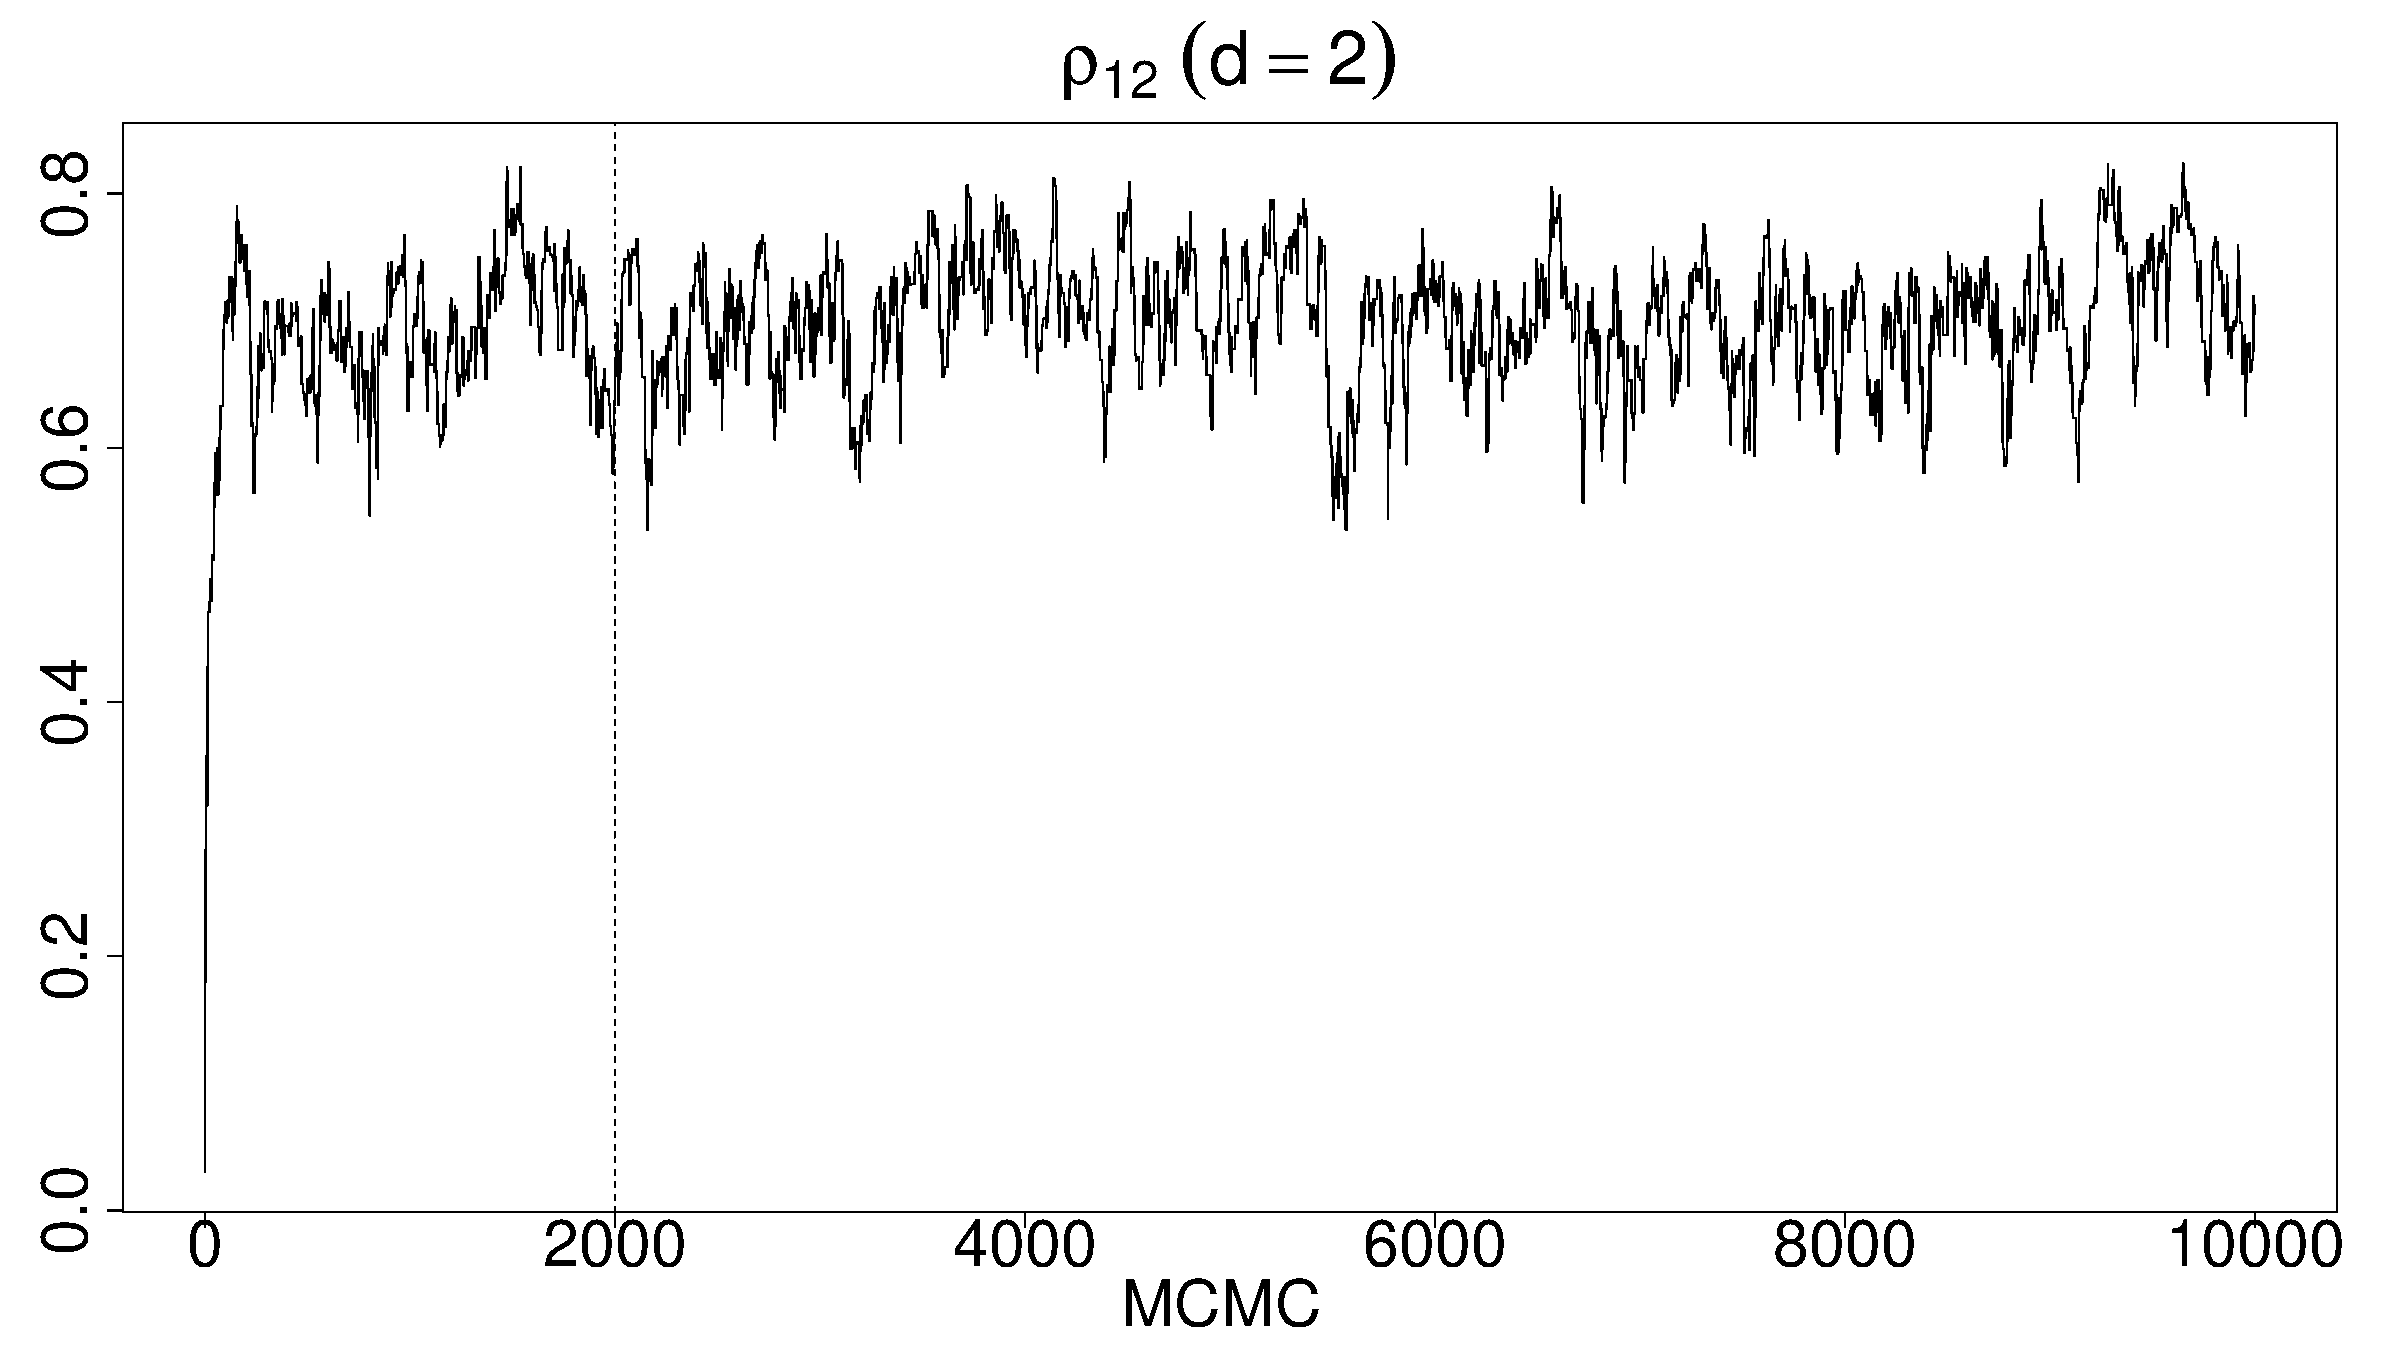
\includegraphics[width=\linewidth]{figures/supplement/rho_subart_friedman1_classification_n_1000_p_10_ntree_100_mvndim_2_nmcmc_10000_nuprop_100.pdf}
\end{subfigure}%
\begin{subfigure}[t]{0.49\textwidth}
    \centering
    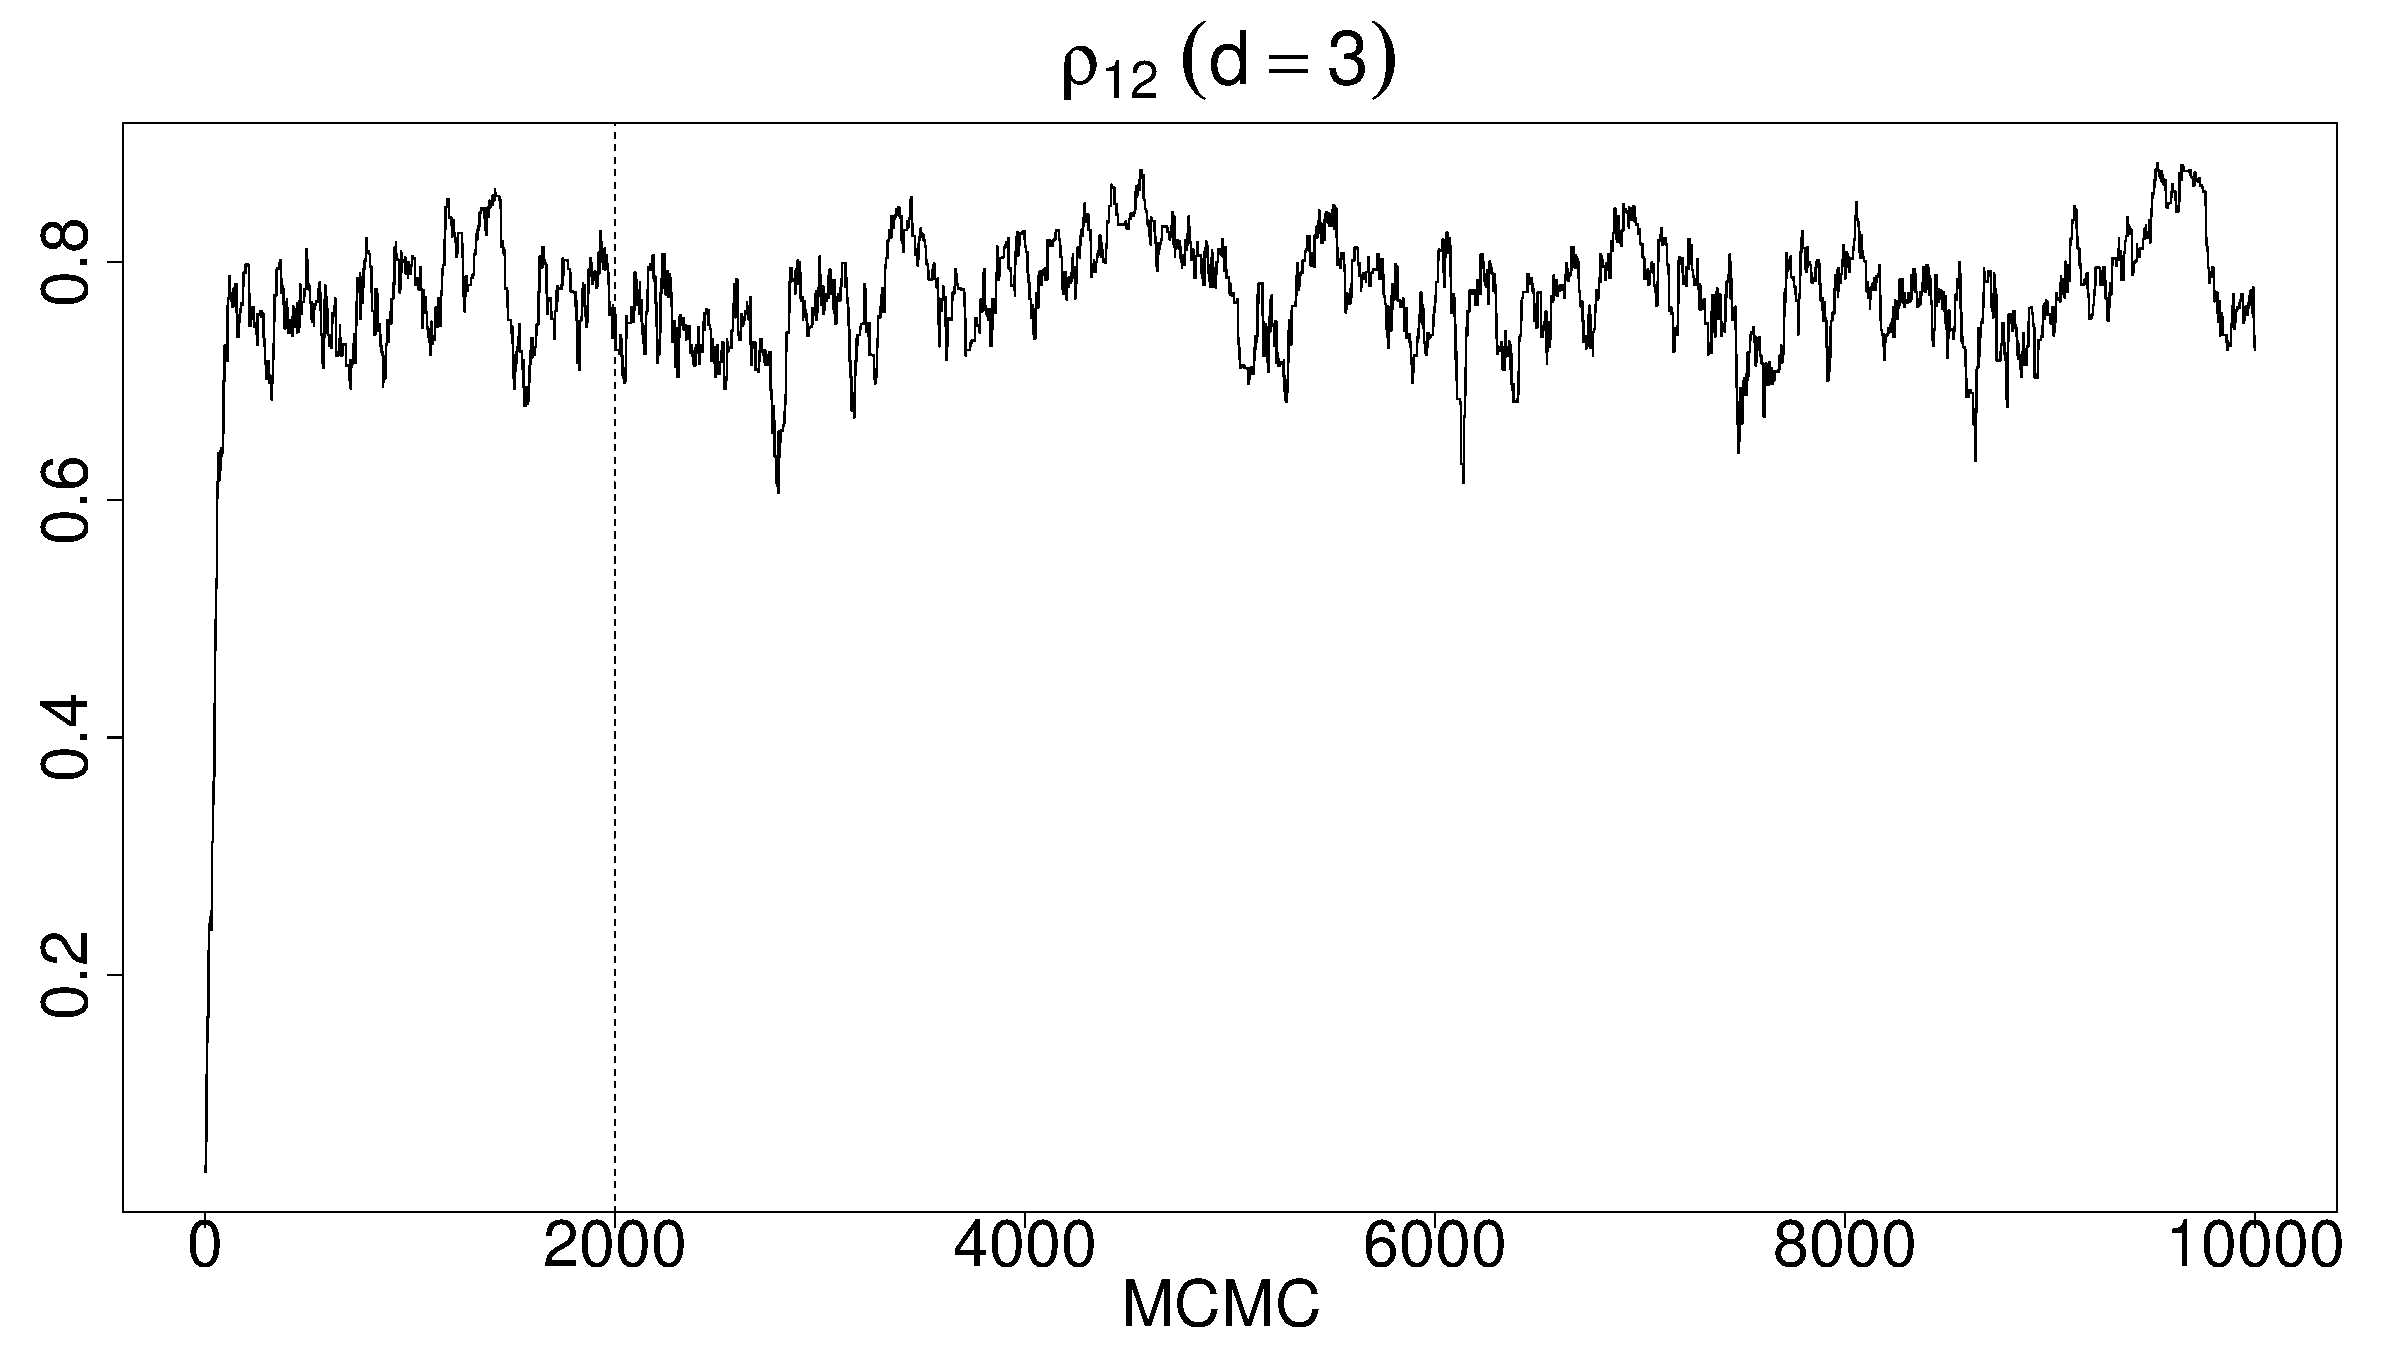
\includegraphics[width=\linewidth]{figures/supplement/rho_subart_friedman1_classification_n_1000_p_10_ntree_100_mvndim_3_nmcmc_10000_nuprop_500.pdf}
\end{subfigure}
\caption{Traceplots of the posterior samples of $\rho_{12}$ considering the Friedman \#2 simulation scenario with $n_{\operatorname{train}}=1000$ and $d=2$ (left) and $d=3$ (right). The dashed vertical line represents the number of iterations used as burn-in.}\label{fig:traceplot_d_23_rho_classification}
\end{figure}%
For completeness, we also show the convergence behaviour of the continuous version of our model for the same $\rho_{12}$ under a randomly chosen replicate of the Friedman \#1 scenario, with $d=\{2,3\}$ and $n_{\operatorname{train}}=1000$, in Figure \ref{fig:traceplot_d_23_rho_regression}. There are evidently no convergence issues in this scenario. Indeed, further examination of traceplots across all relevant simulation experiments and configurations of sample size and dimensionality suggest that our sampler is adequate in the case of continuous responses.
\begin{figure}[H]
\centering
\begin{subfigure}[t]{0.49\textwidth}
    \centering
    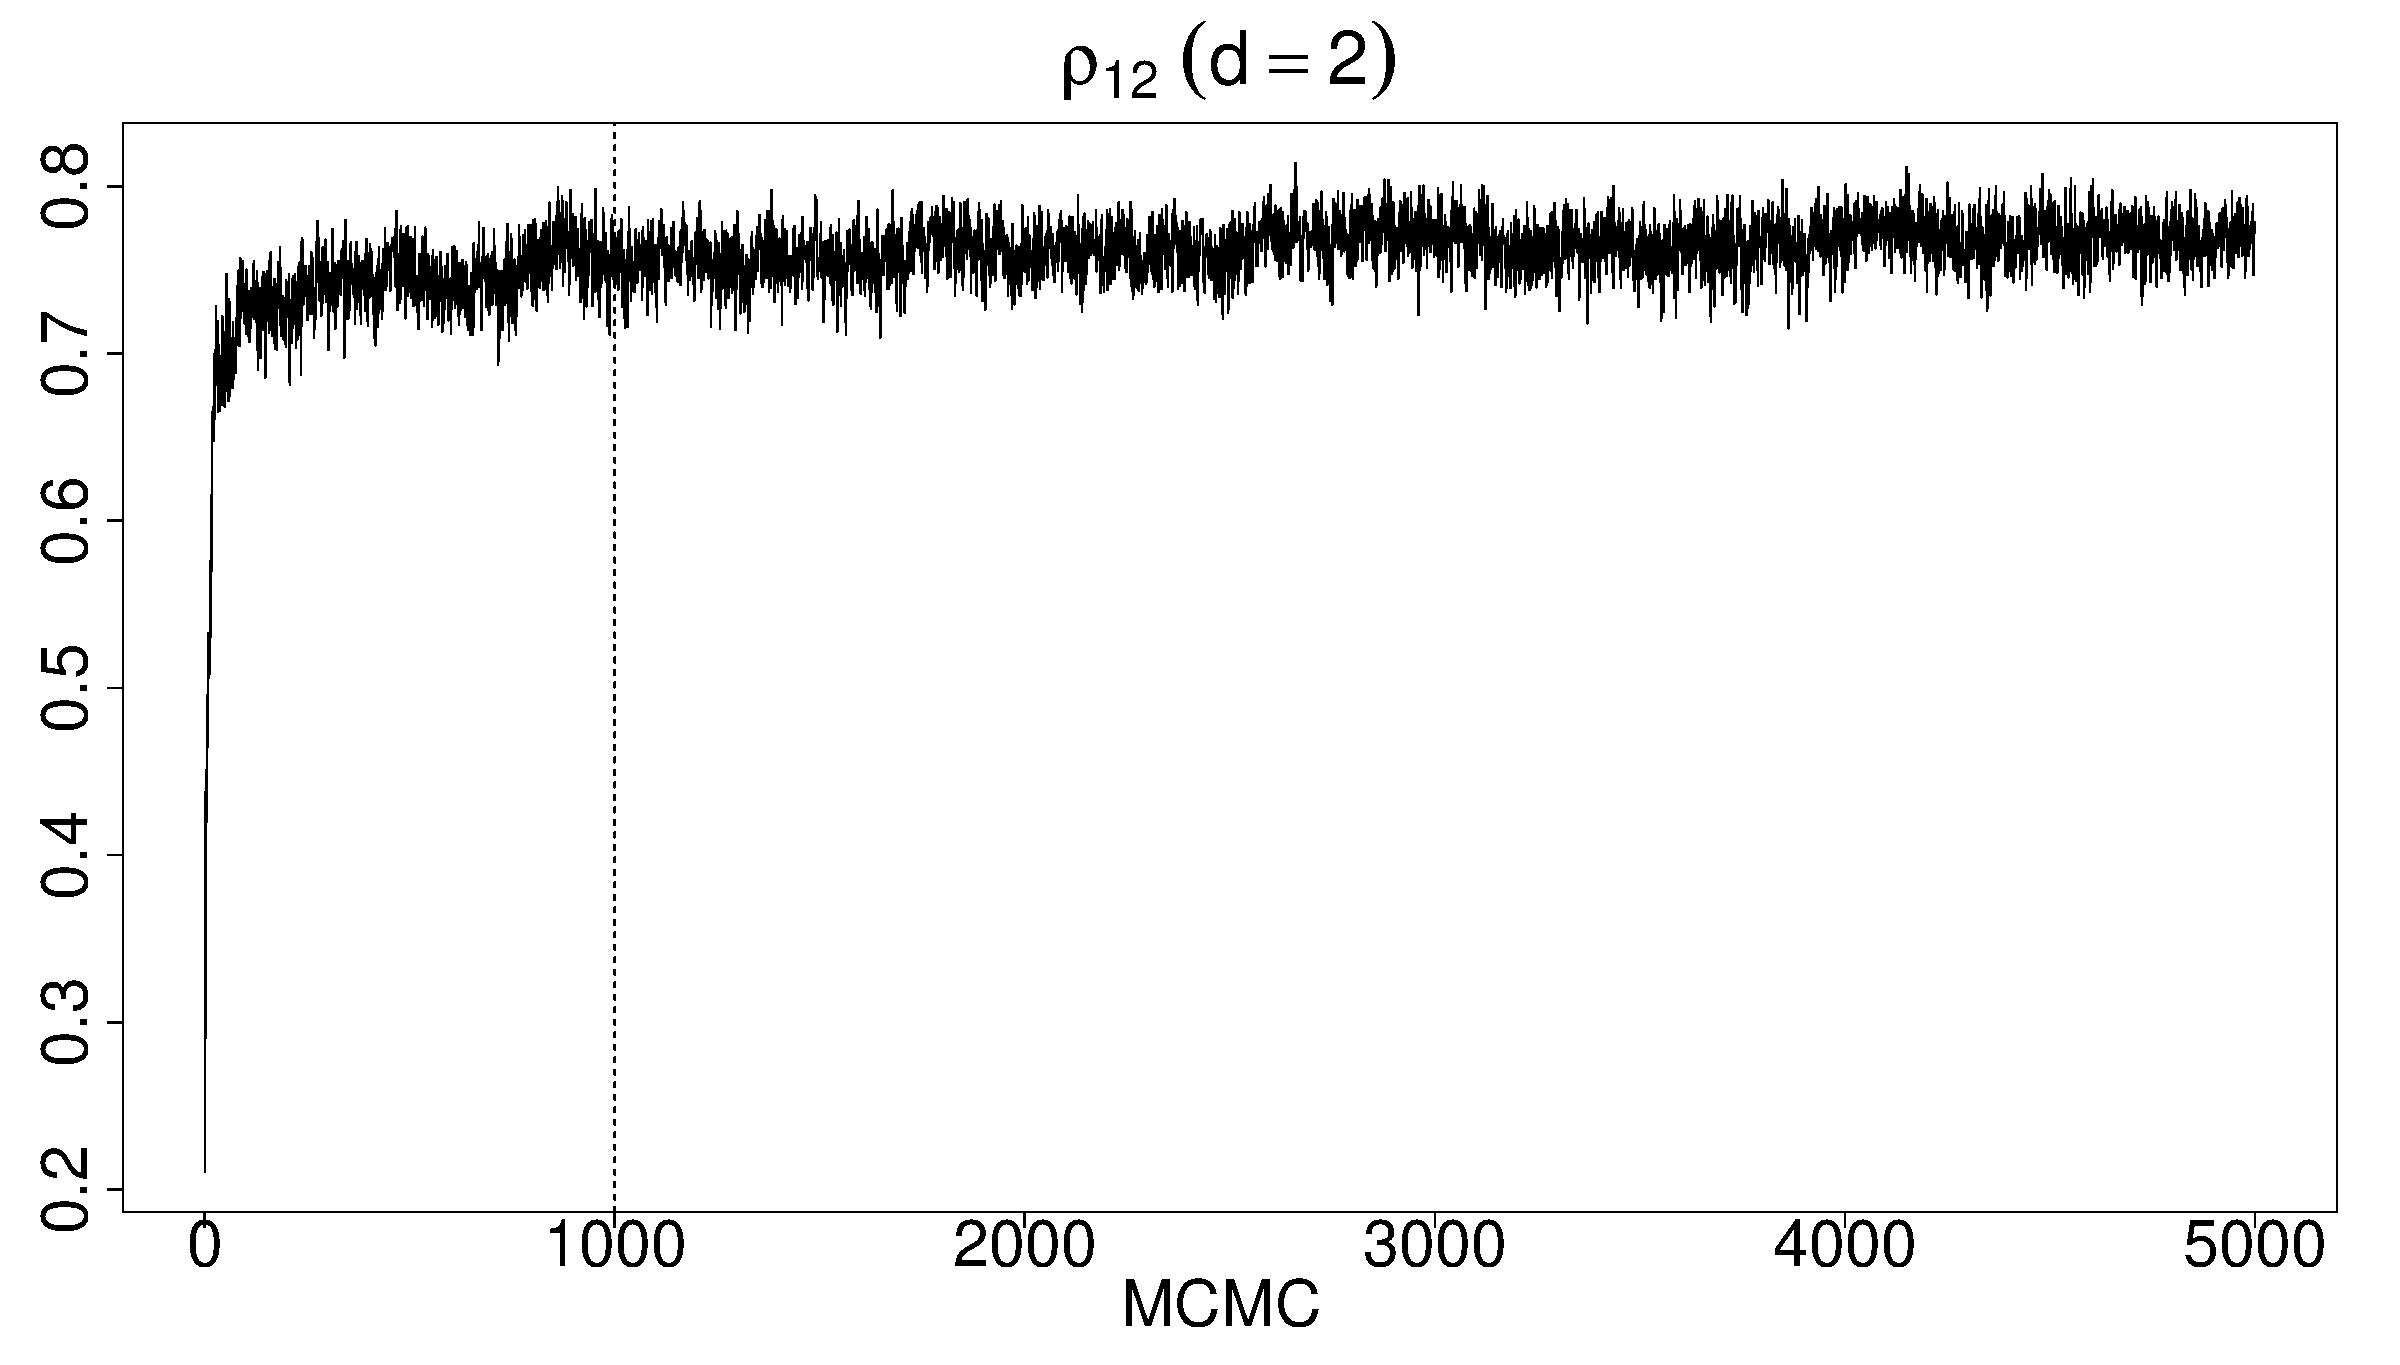
\includegraphics[width=\linewidth]{figures/supplement/rho_subart_friedman1_regression_n_1000_p_10_ntree_100_mvndim_2_nmcmc_5000_nuprop_100.pdf}
\end{subfigure}%
\begin{subfigure}[t]{0.49\textwidth}
    \centering
    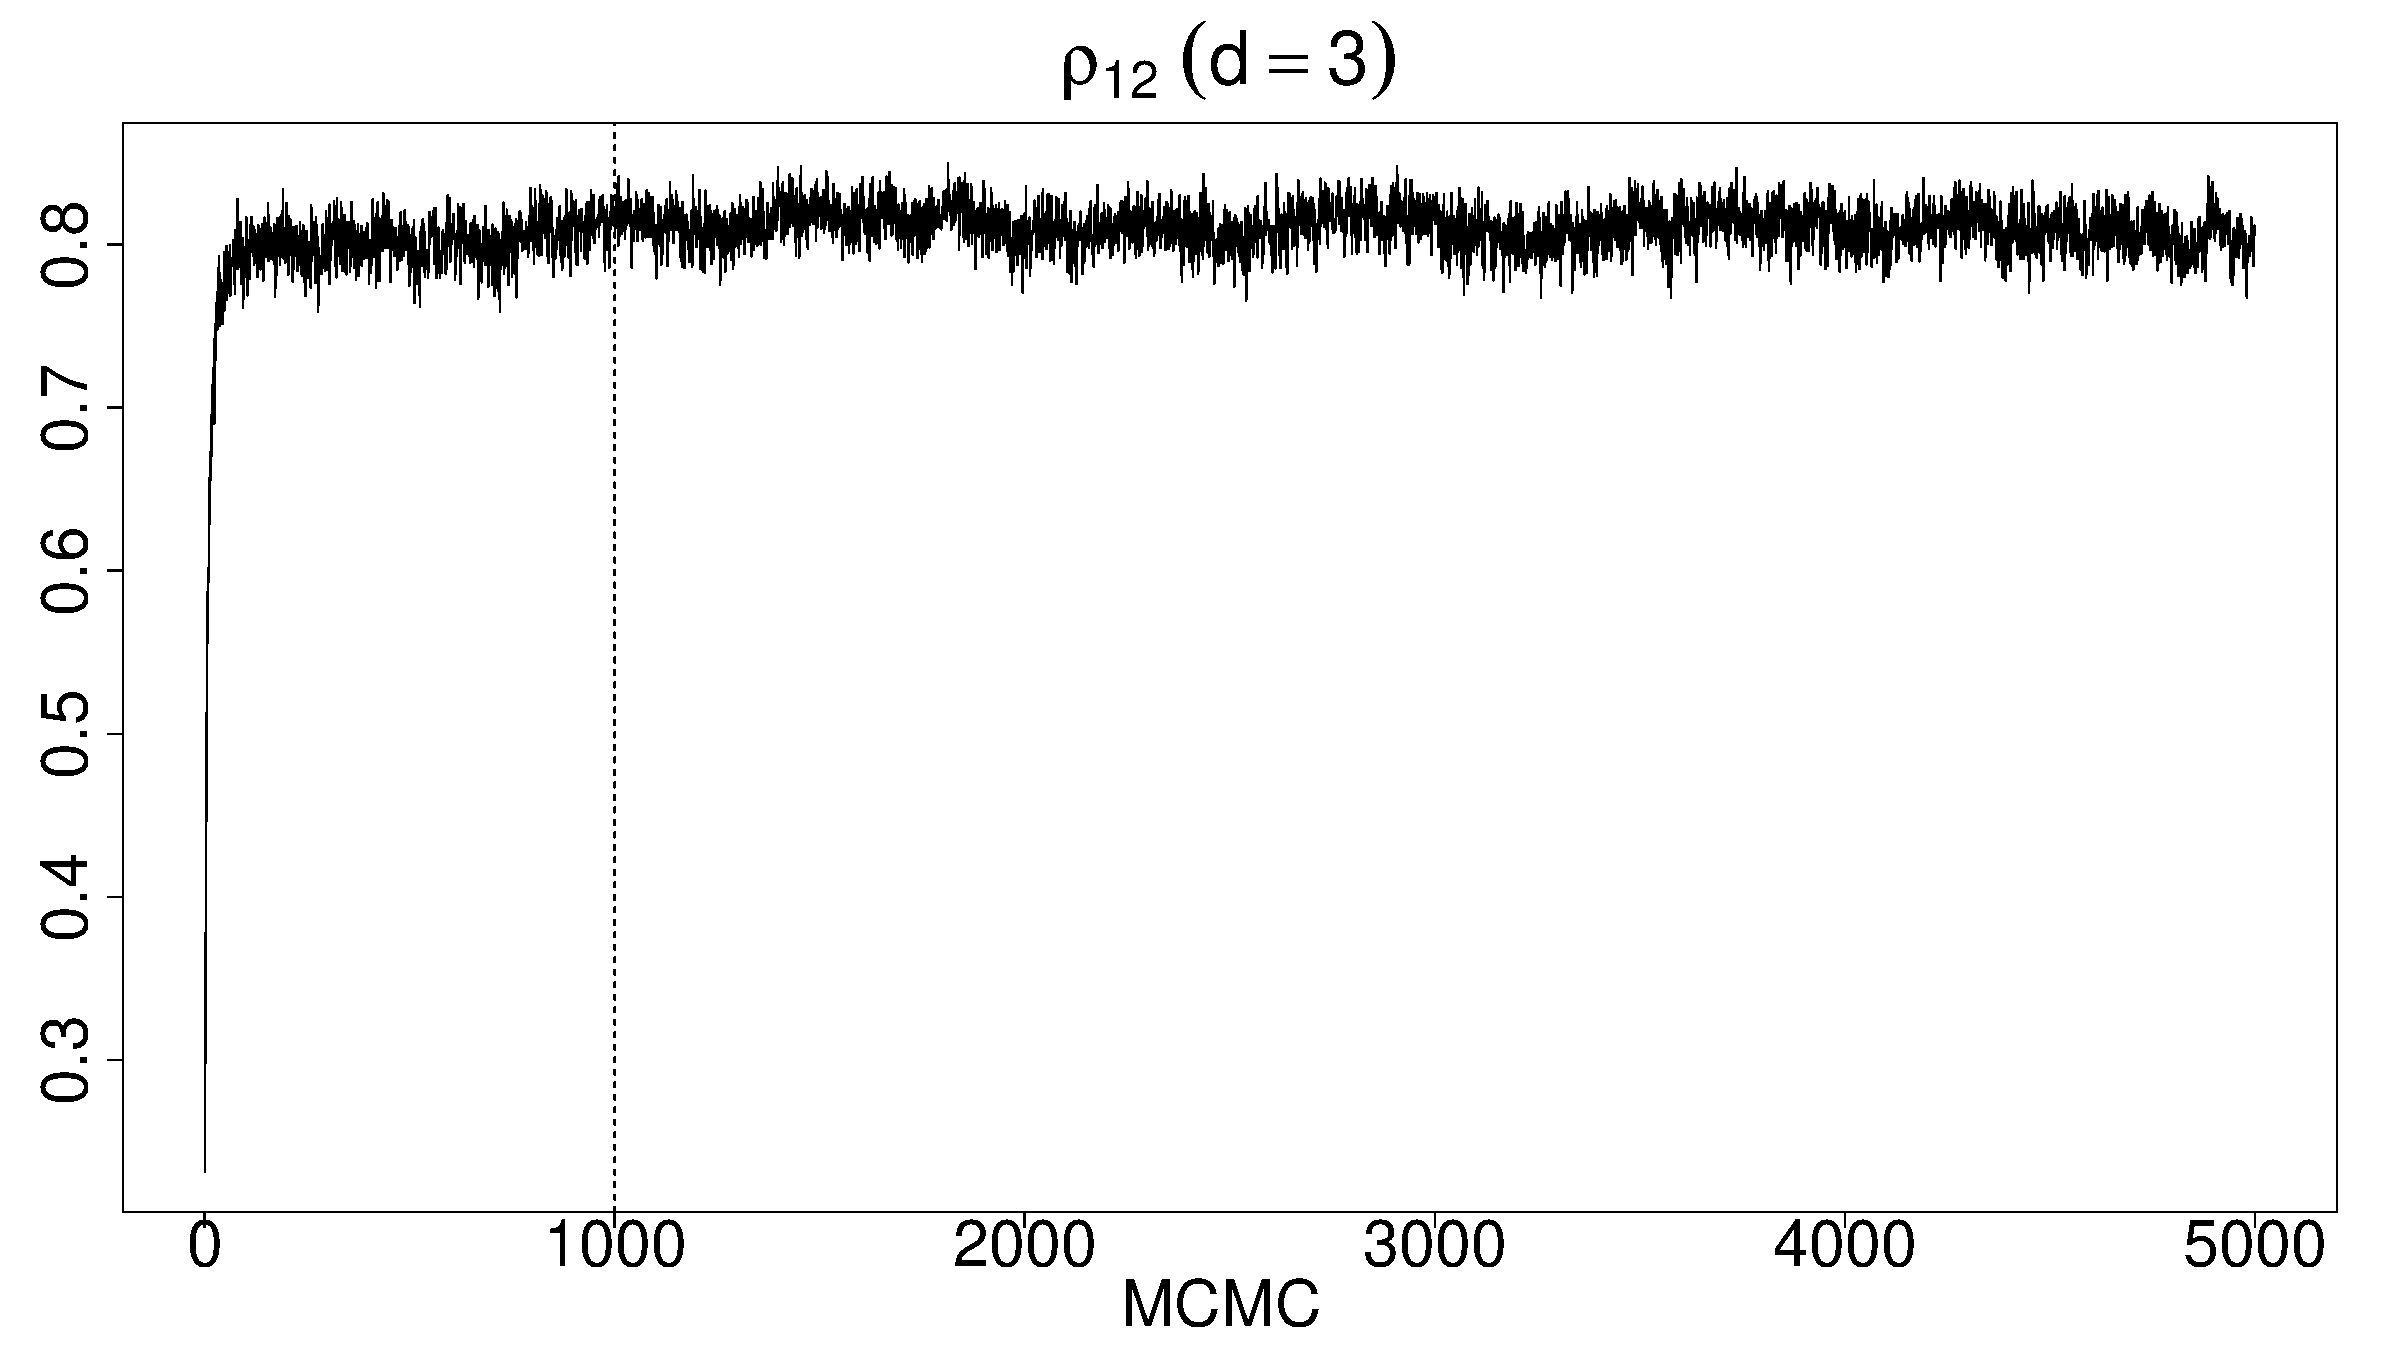
\includegraphics[width=\linewidth]{figures/supplement/rho_subart_friedman1_regression_n_1000_p_10_ntree_100_mvndim_3_nmcmc_5000_nuprop_500.pdf}
\end{subfigure}
\caption{Traceplots of the posterior samples of $\rho_{12}$ considering the Friedman \#1 simulation scenario with $n_{\operatorname{train}}=1000$ and $d=2$ (left) and $d=3$ (right). The dashed vertical line represents the number of iterations used as burn-in.}\label{fig:traceplot_d_23_rho_regression}
\end{figure}

\section{Additional Friedman simulation experiments}
\setcounter{figure}{0}
\setcounter{table}{0}
\label{app:friedman}

In order to evaluate the performance of suBART against its competitors, we conducted experiments outlined in Section \ref{sec:simstudies}, where we varied $n_{\operatorname{train}} = n_{\operatorname{test}} = \{250,500,1000\}$ and $d = \{2,3\}$. This Appendix summarises the remaining results omitted from the main paper, for different configurations of sample size and dimensionality of the outcome. %along with the results of an additional simulation design described below. More specifically, the remainder of this Appendix shows the boxplots of RMSE and PI coverage and associated tables of results for all configurations of sample size and dimensionality of the outcome, across both simulation scenarios, which were not previously shown in the main body of the paper. 
Recall that mvBART is excluded wherever $d=3$, due to the limitations of the \texttt{skewBART} package.
Overall, the findings illustrated in the boxplots below align with the conclusions drawn in Section \ref{sec:simstudies}. In particular, suBART exhibits reasonable performance metrics for both continuous (Friedman \#1) and binary (Friedman \#2) outcome scenarios, either matching or surpassing its tree-based model counterparts. Notably, suBART outperforms the linear BayesSUR across all scenarios, with the exception of the responses whose dependence on the predictors is linear. Additionally, we provide a summary of the estimated correlation parameters through tables displaying the RMSE and $50\%$ CI coverage for all $\rho_{kj}$ where $j\neq k$. Across all scenarios, suBART consistently approaches the true values and provides credible intervals with proper coverage rates.
\begin{figure}[H]
    \centering
    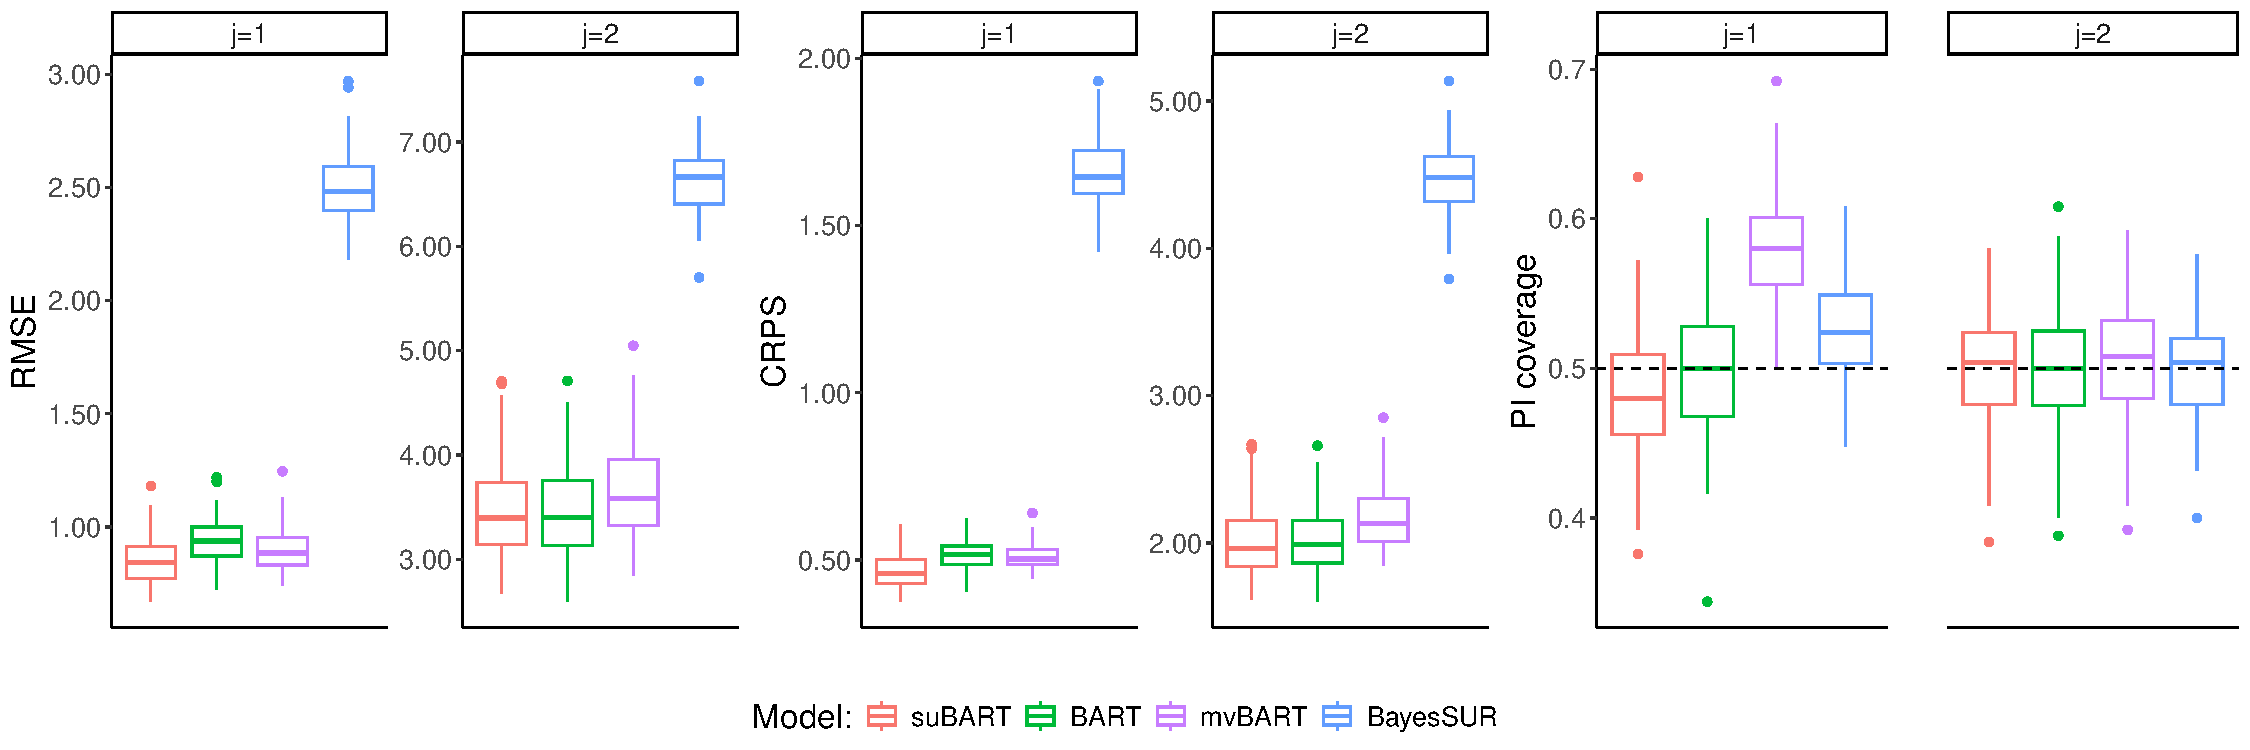
\includegraphics[width=\textwidth]{figures/supplement/friedman1_regression_250_2.pdf}
    \caption{Simulation results for Friedman \#1 under the suBART, BART, mvBART, and BayesSUR models (from left to right) with $n_{\operatorname{train}} = n_{\operatorname{test}}=250 $ and $d = 2$.}
    \label{fig:sim_reg_friedman_one_250_2d}
\end{figure}
\begin{figure}[H]
    \centering
    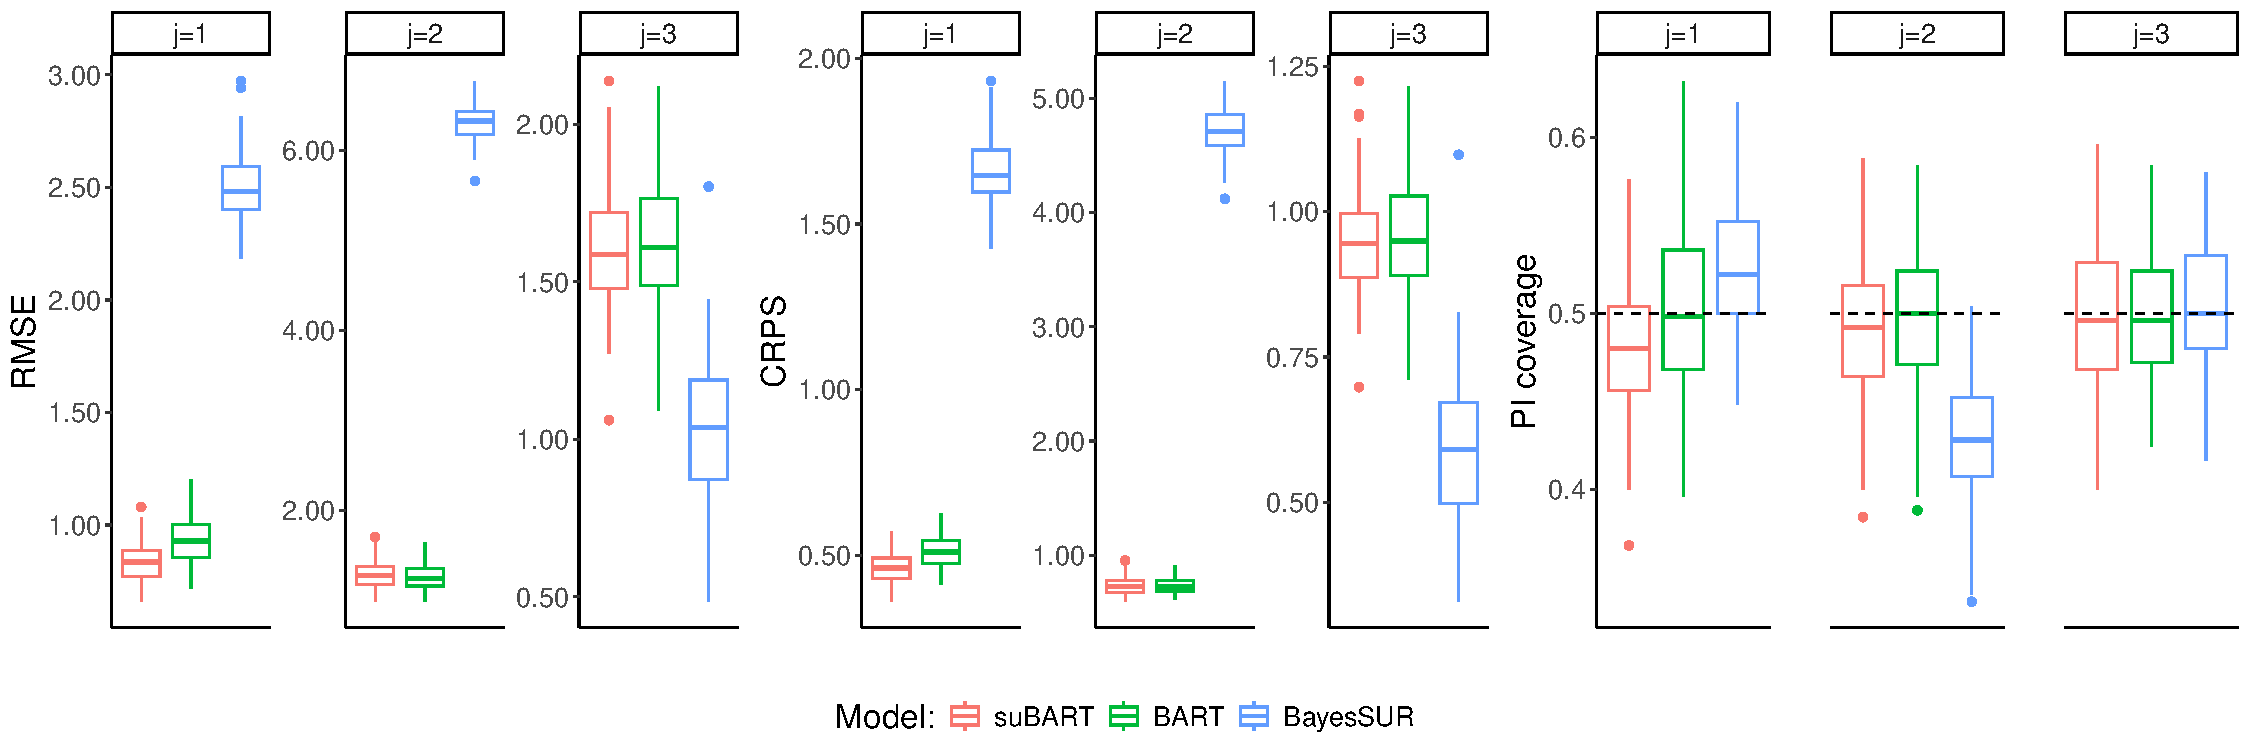
\includegraphics[width=\textwidth]{figures/supplement/friedman1_regression_250_3.pdf}
    \caption{Simulation results for Friedman \#1 under the suBART, BART, and BayesSUR models (from left to right) with $n_{\operatorname{train}} = n_{\operatorname{test}}=250 $ and $d = 3$.}
    \label{fig:sim_reg_friedman_one_250_3d}
\end{figure}
\begin{figure}[H]
    \centering
    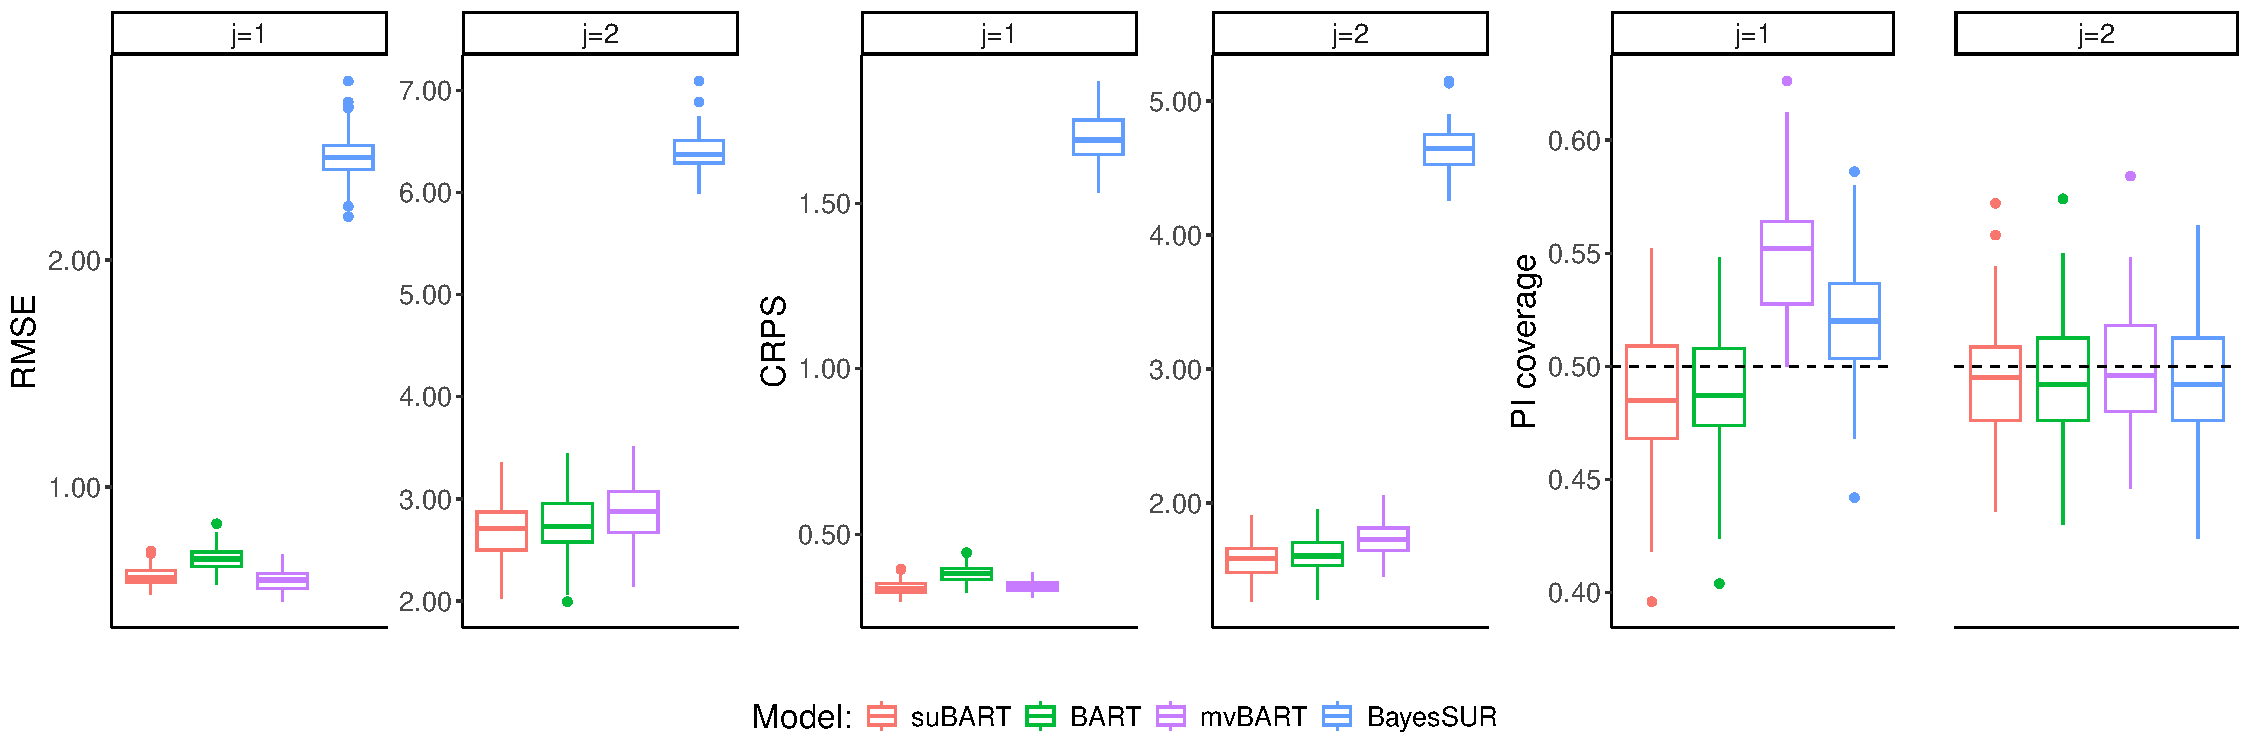
\includegraphics[width=\textwidth]{figures/supplement/friedman1_regression_500_2.pdf}
    \caption{Simulation results for Friedman \#1 under the suBART, BART, mvBART, and BayesSUR models (from left to right) with $n_{\operatorname{train}} = n_{\operatorname{test}}=500 $ and $d = 2$.}
    \label{fig:sim_reg_friedman_one_500_2d}
\end{figure}
\begin{figure}[H]
    \centering
    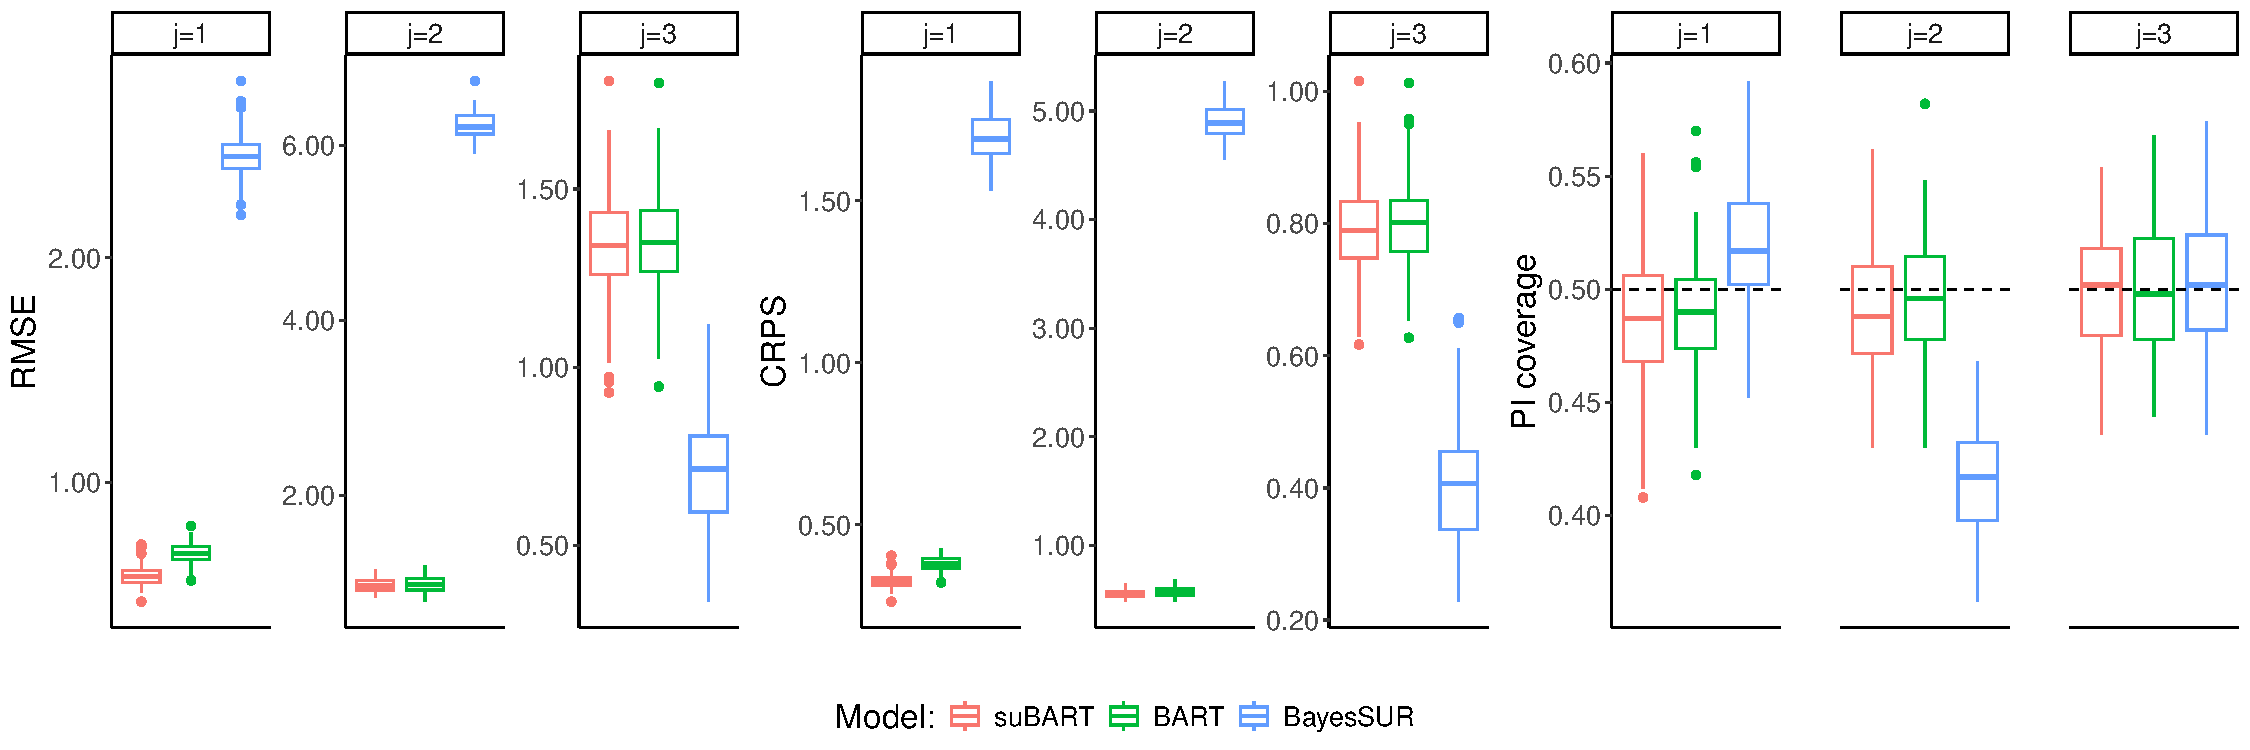
\includegraphics[width=\textwidth]{figures/supplement/friedman1_regression_500_3.pdf}
    \caption{Simulation results for Friedman \#1 under the suBART, BART, and BayesSUR models (from left to right) with $n_{\operatorname{train}} = n_{\operatorname{test}}=500 $ and $d = 3$.}
    \label{fig:sim_reg_friedman_one_500_3d}
\end{figure}
\begin{figure}[H]
    \centering
    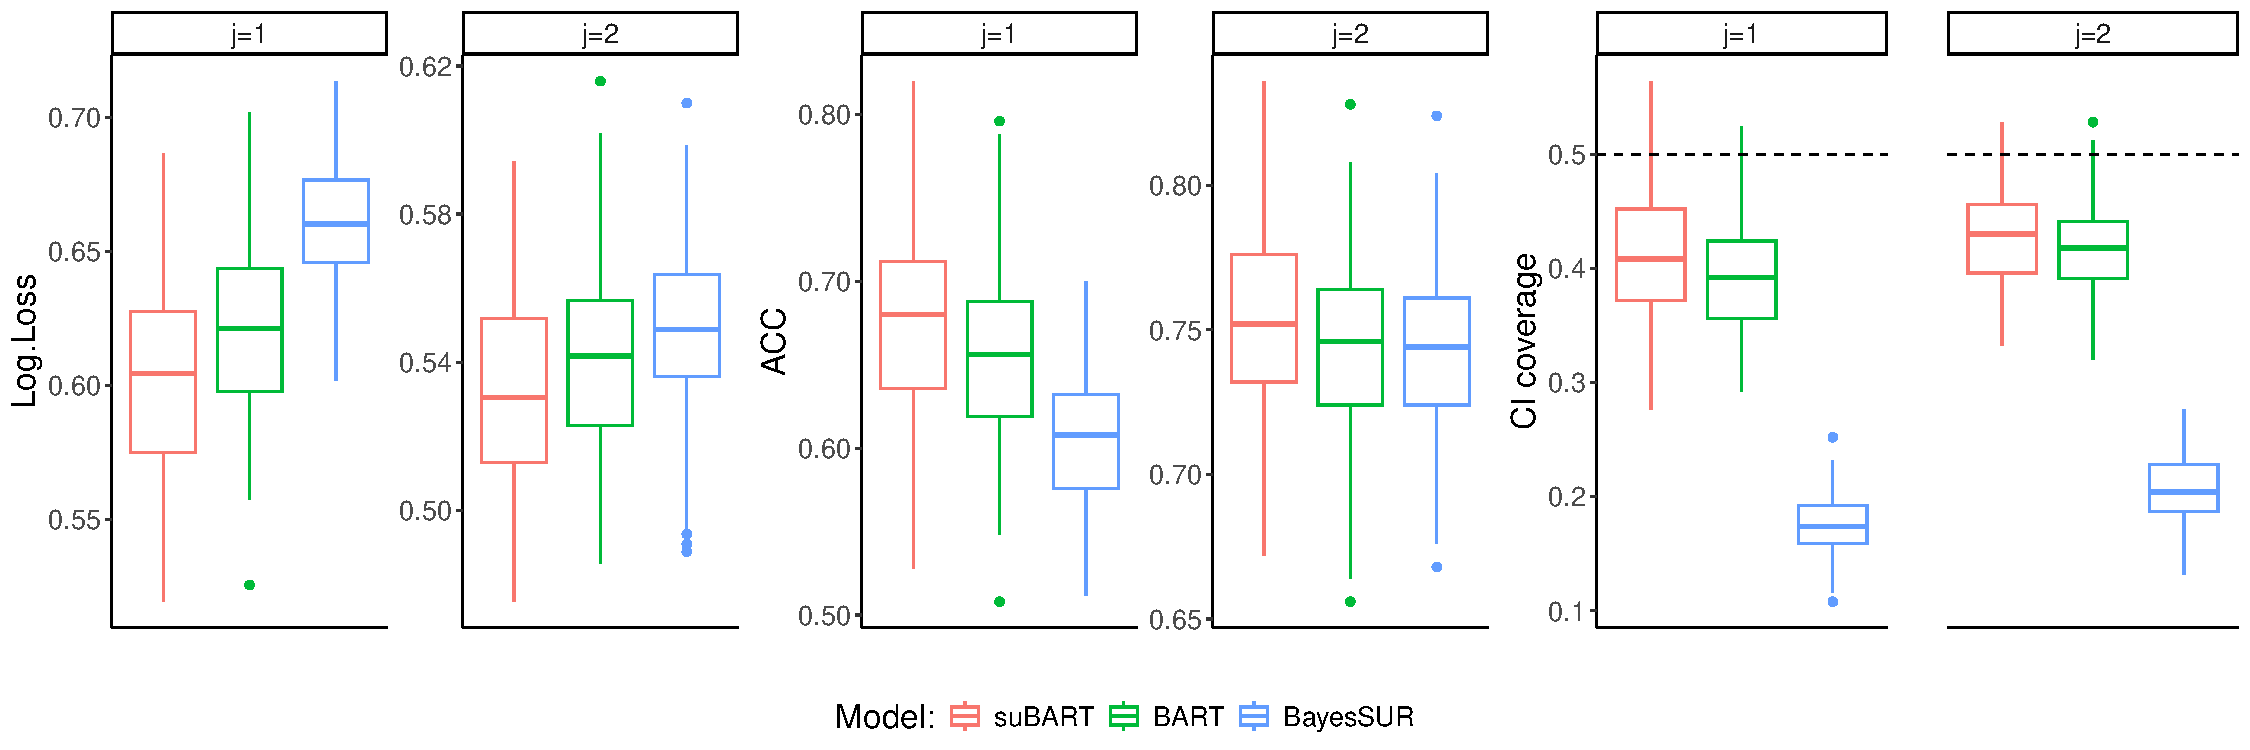
\includegraphics[width=\textwidth]{figures/supplement/friedman1_classification_250_2.pdf}
    \caption{Simulation results for Friedman \#2 under the suBART, BART, and BayesSUR models (from left to right) with $n_{\operatorname{train}} = n_{\operatorname{test}}=250 $ and $d = 2$.}
    \label{fig:sim_class_friedman_one_250_2d}
\end{figure}
\begin{figure}[H]
    \centering
    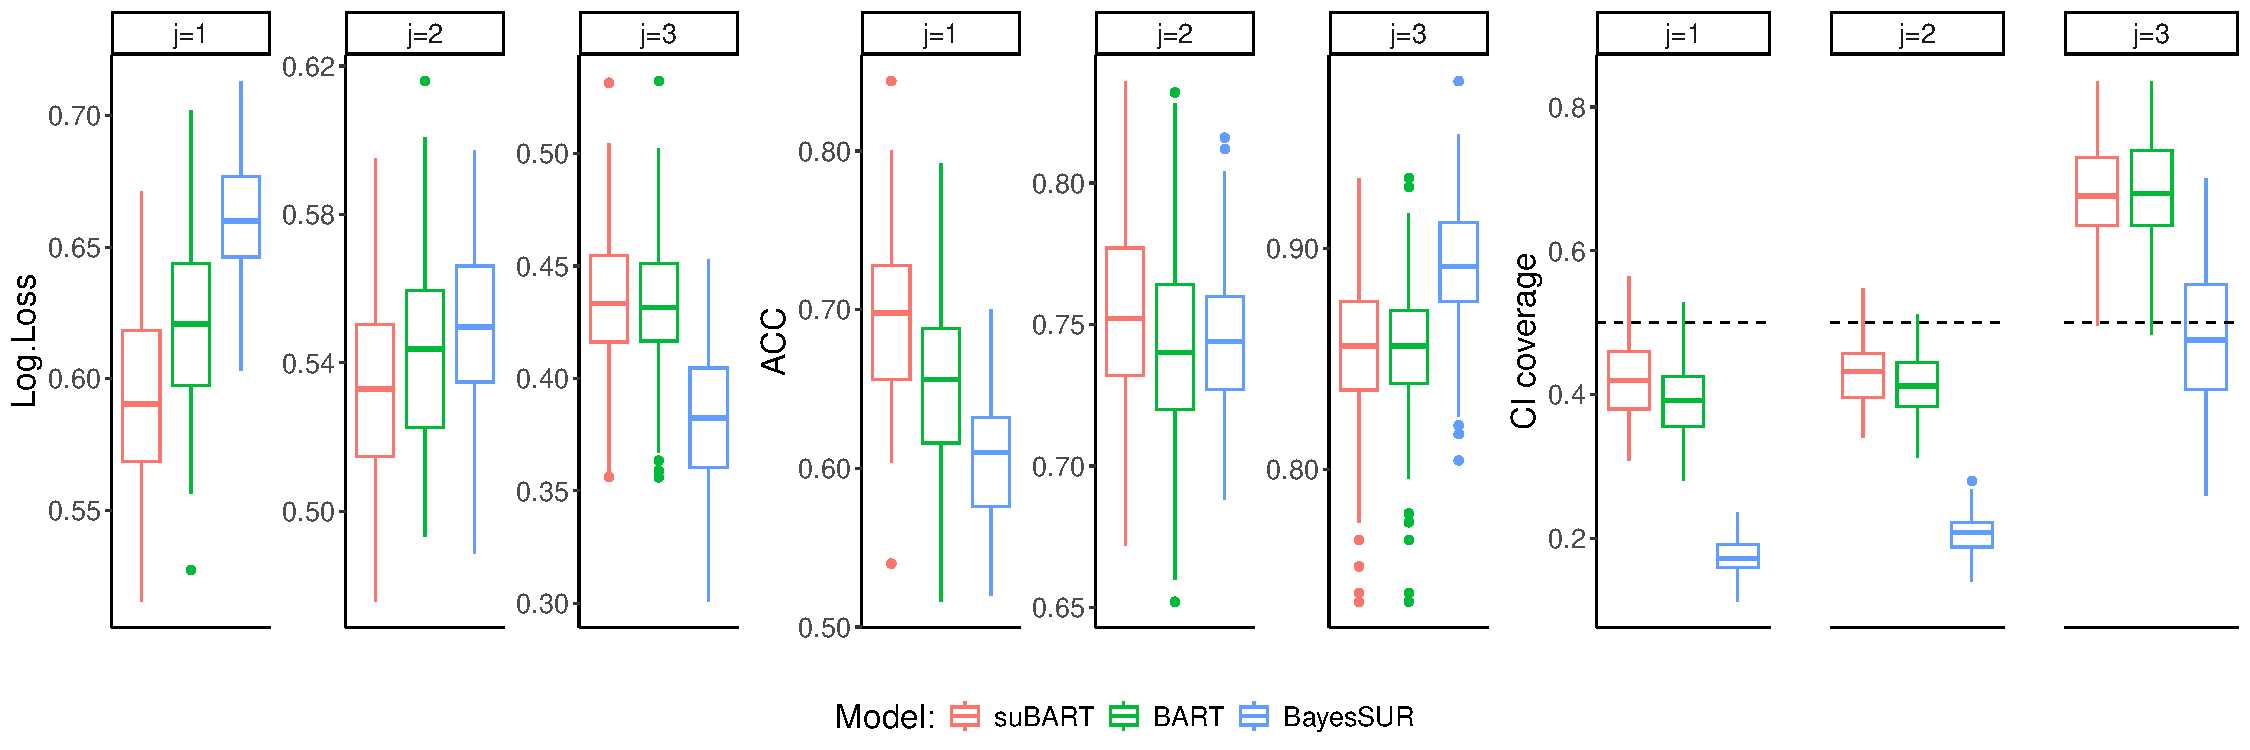
\includegraphics[width=\textwidth]{figures/supplement/friedman1_classification_250_3.pdf}
    \caption{Simulation results for Friedman \#2 under the suBART, BART, and BayesSUR models (from left to right) with $n_{\operatorname{train}} = n_{\operatorname{test}}=250 $ and $d = 3$.}
    \label{fig:sim_class_friedman_one_250_3d}
\end{figure}
\begin{figure}[H]
    \centering
    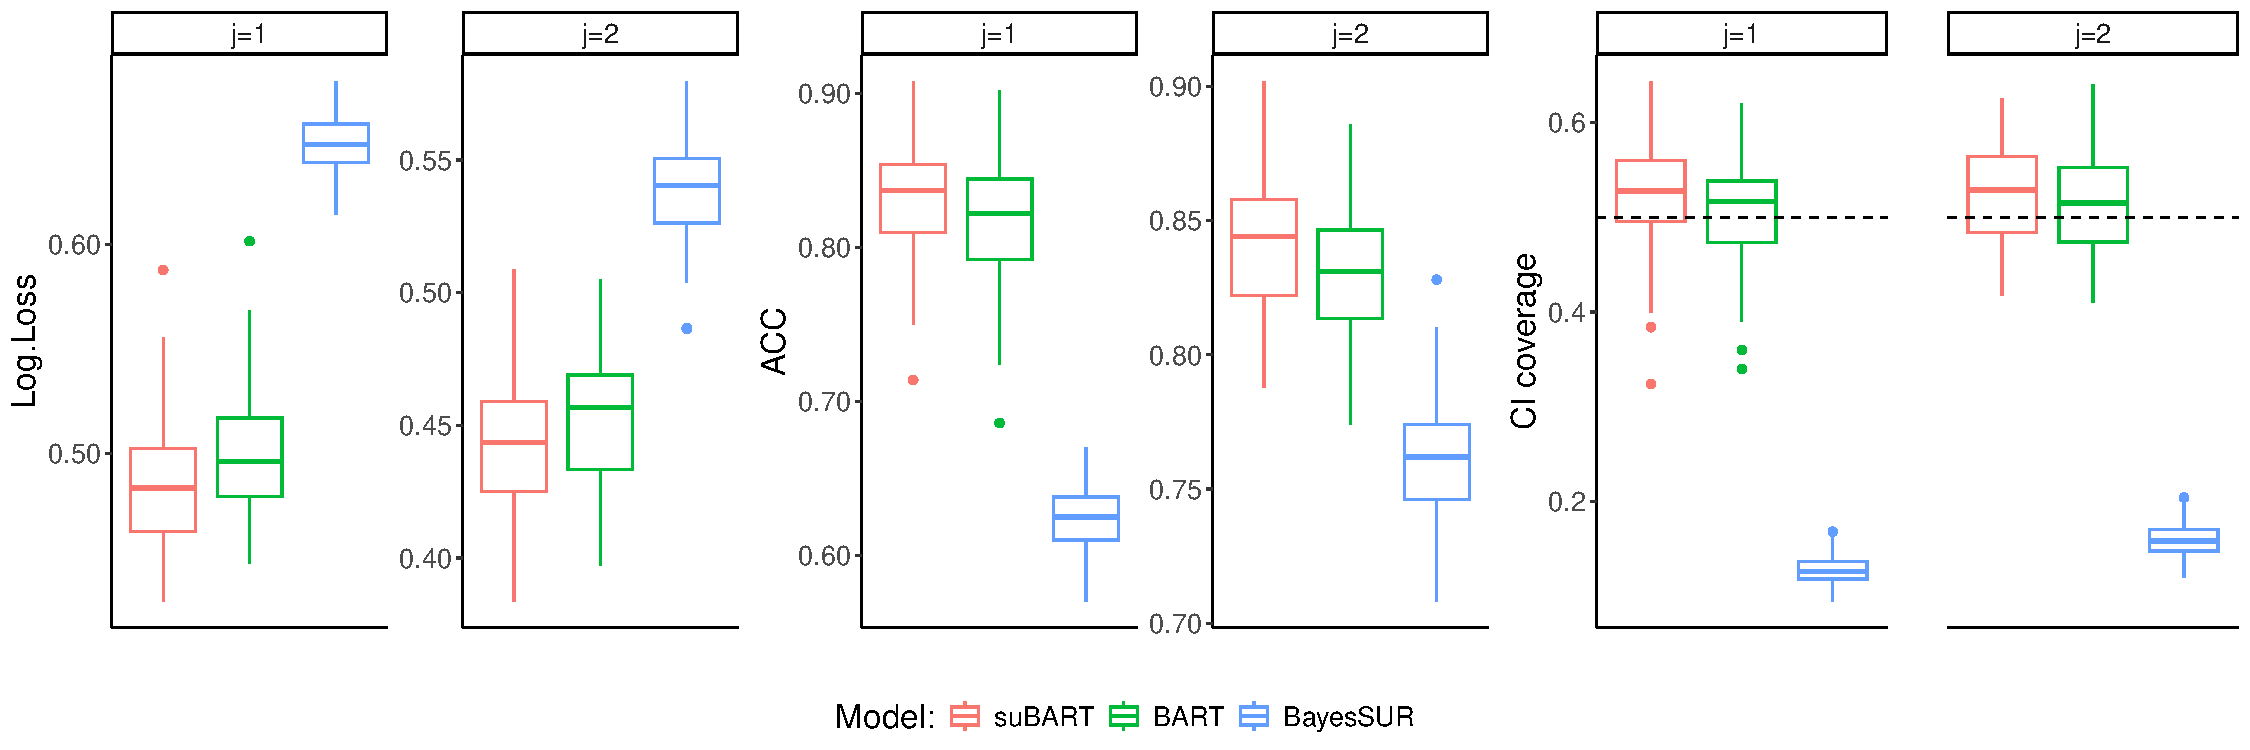
\includegraphics[width=\textwidth]{figures/supplement/friedman1_classification_500_2.pdf}
    \caption{Simulation results for Friedman \#2 under the suBART, BART, and BayesSUR models (from left to right) with $n_{\operatorname{train}} = n_{\operatorname{test}}=500 $ and $d = 2$.}
    \label{fig:sim_class_friedman_one_500_2d}
\end{figure}
\begin{figure}[H]
    \centering
    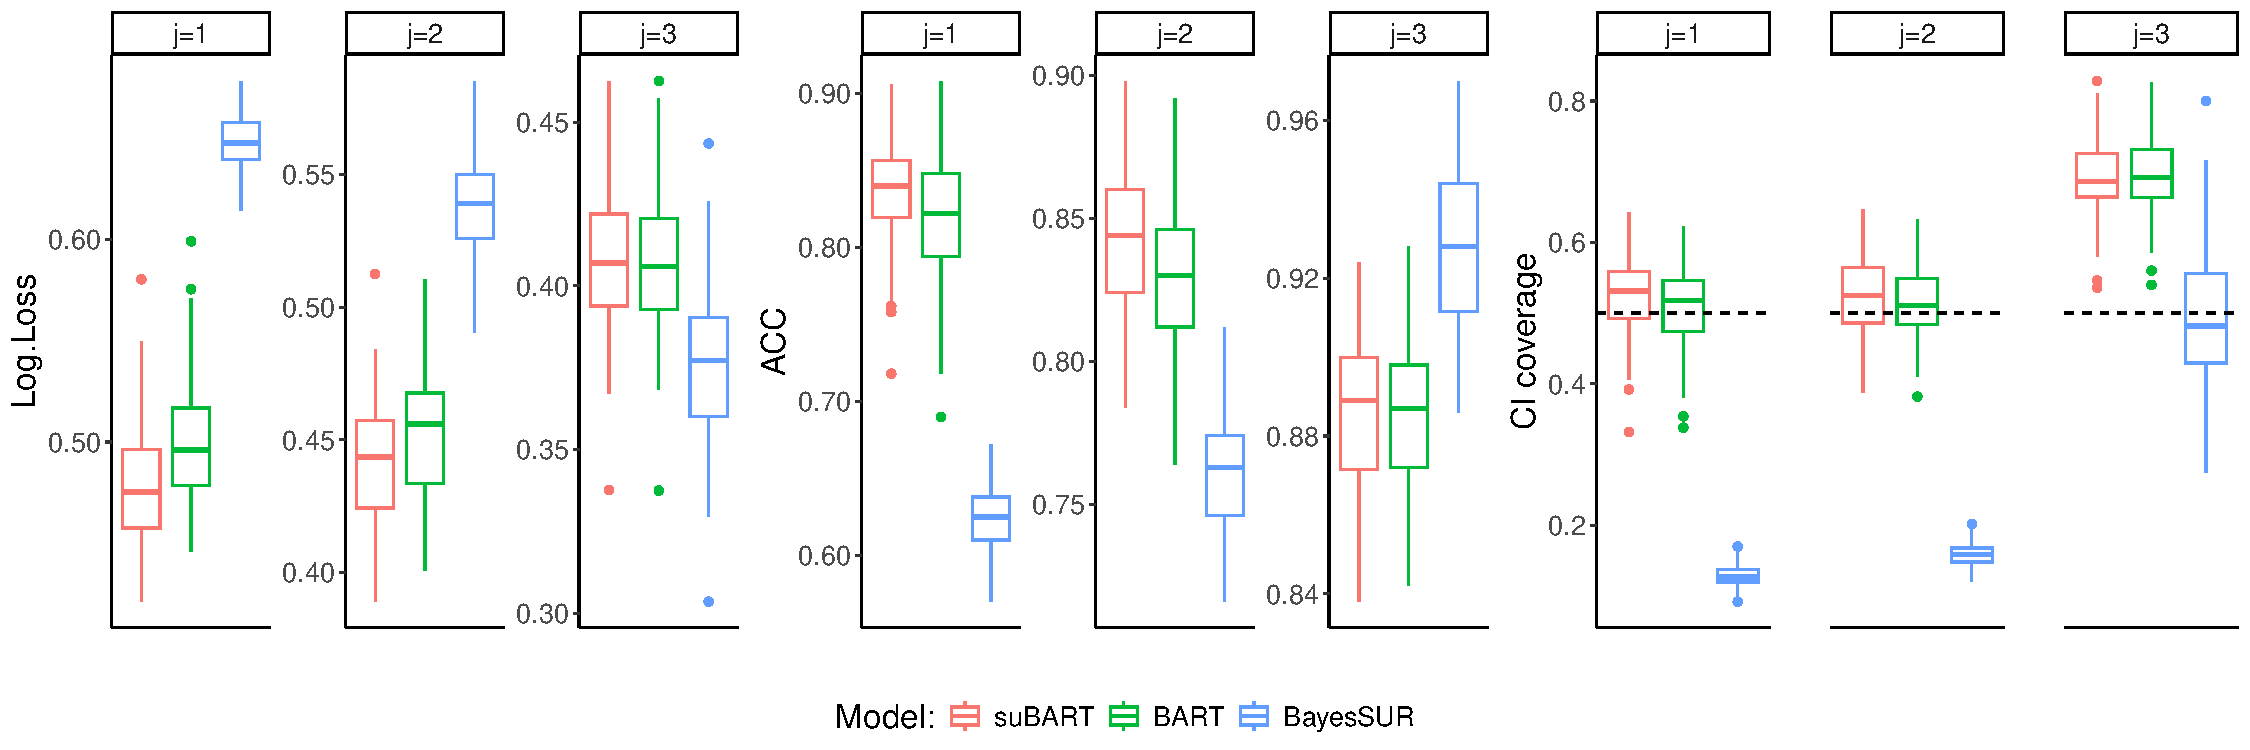
\includegraphics[width=\textwidth]{figures/supplement/friedman1_classification_500_3.pdf}
    \caption{Simulation results for Friedman \#2 under the suBART, BART, and BayesSUR models (from left to right) with $n_{\operatorname{train}} = n_{\operatorname{test}}=500 $ and $d = 3$.}
    \label{fig:sim_class_friedman_one_500_3d}
\end{figure}
\begin{figure}[H]
    \centering
    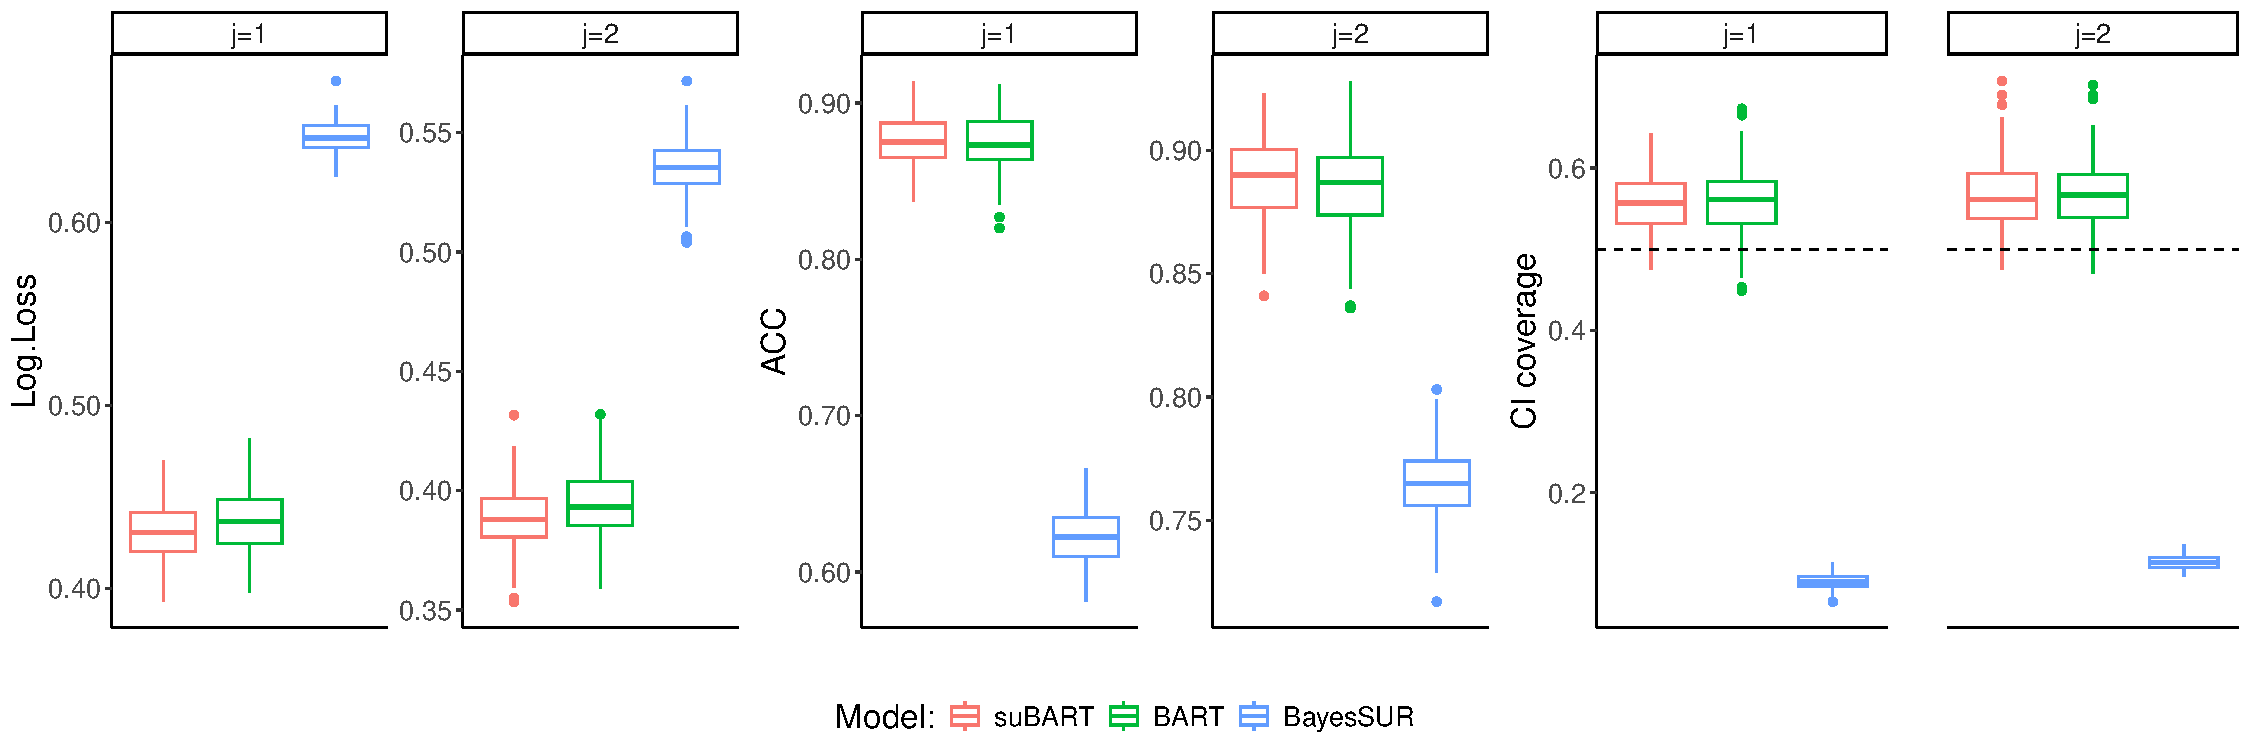
\includegraphics[width=\textwidth]{figures/supplement/friedman1_classification_1000_2.pdf}
    \caption{Simulation results for Friedman \#2 under the suBART, BART, and BayesSUR models (from left to right) with $n_{\operatorname{train}} = n_{\operatorname{test}}=1000 $ and $d = 2$.}
    \label{fig:sim_class_friedman_one_1000_2d}
\end{figure}\vspace{-1em}%
\begin{table}[H]
\centering
\caption{RMSE and coverage of a $50\%$ CI for $\sigma_j$ and ${\rho}_{jk}$  for Friedman \#1 with $n_{\operatorname{train}} = n_{\operatorname{test}} =250$.}
\label{tab:sim_corr_fried_one_combined_250}
\begin{tabular}{llcccccccc}
\hline
\small
&& \multicolumn{4}{c}{\textbf{RMSE}} & \multicolumn{4}{c}{\textbf{CI coverage}} \\
&& \textbf{suBART} & \textbf{BART} & \textbf{mvBART} & \textbf{BayesSUR} & \textbf{suBART} & \textbf{BART} & \textbf{mvBART} & \textbf{BayesSUR} \\
\hline
\multirow{3}{*}{$d=2$}&{$\sigma_1$} & $0.08$ & $0.09$ & $0.08$ & $1.62$ & $0.28$ & $0.38$ & $0.46$ & $0.00$ \\
&{$\sigma_2$} & $0.58$ & $0.63$ & $0.82$ & $1.87$ & $0.30$ & $0.26$ & $0.15$ & $0.00$ \\
&{$\rho_{12}$} & $0.06$ & --- & $0.04$ & $0.31$ & $0.28$ & --- & $0.59$ & $0.00$ \\ 
\hline
\multirow{6}{*}{$d=3$}&{$\sigma_1$} & $0.06$ & $0.08$ & --- & $1.62$ & $0.46$ & $0.41$ & --- & $0.00$ \\
&{$\sigma_2$} & $0.26$ & $0.32$ & --- & $4.18$ & $0.10$ & $0.03$ & --- & $0.00$ \\
&{$\sigma_3$} & $0.35$ & $0.35$ & --- & $0.20$ & $0.27$ & $0.25$ & --- & $0.47$ \\
&{$\rho_{12}$} & $0.06$ & --- & --- & $0.35$ & $0.16$ & --- & --- & $0.00$ \\ 
&{$\rho_{13}$} & $0.06$ & --- & --- & $0.31$ & $0.40$ & --- & --- & $0.00$ \\
&{$\rho_{23}$} & $0.06$ & --- & --- & $0.16$ & $0.47$ & --- & --- & $0.03$ \\ 
\end{tabular}
\end{table}\vspace{-1em}%
\begin{table}[H]
\centering
\caption{RMSE and coverage of a $50\%$ CI for $\sigma_j$ and ${\rho}_{jk}$  for Friedman \#1 with $n_{\operatorname{train}} = n_{\operatorname{test}} =500$.}
\label{tab:sim_corr_fried_one_combined_500}
\begin{tabular}{llcccccccc}
\hline
\small
&& \multicolumn{4}{c}{\textbf{RMSE}} & \multicolumn{4}{c}{\textbf{CI coverage}} \\
& & \textbf{suBART} & \textbf{BART} & \textbf{mvBART} & \textbf{BayesSUR} & \textbf{suBART} & \textbf{BART} & \textbf{mvBART} & \textbf{BayesSUR} \\
\hline
\multirow{3}{*}{$d=2$}&{$\sigma_1$} & $0.05$ & $0.07$ & $0.06$ & $1.61$ & $0.35$ & $0.09$ & $0.20$ & $0.00$ \\
&{$\sigma_2$} & $0.44$ & $0.48$ & $0.56$ & $1.75$ & $0.30$ & $0.28$ & $0.18$ & $0.00$ \\
&{$\rho_{12}$} & $0.03$ & --- & $0.02$ & $0.32$ & $0.38$ & --- & $0.58$ & $0.00$ \\ 
\hline
\multirow{6}{*}{$d=3$}&{$\sigma_1$} & $0.04$ & $0.07$ & --- & $1.61$ & $0.41$ & $0.12$ & --- & $0.00$ \\
&{$\sigma_2$} & $0.14$ & $0.20$ & --- & $4.15$ & $0.18$ & $0.08$ & --- & $0.00$ \\
&{$\sigma_3$} & $0.25$ & $0.26$ & --- & $0.12$ & $0.17$ & $0.17$ & --- & $0.58$ \\
&{$\rho_{12}$} & $0.03$ & --- & --- & $0.35$ & $0.30$ & --- & --- & $0.00$ \\ 
&{$\rho_{13}$} & $0.03$ & --- & --- & $0.31$ & $0.50$ & --- & --- & $0.00$ \\
&{$\rho_{23}$} & $0.04$ & --- & --- & $0.16$ & $0.58$ & --- & --- & $0.00$ \\ 
\end{tabular}
\end{table}\vspace{-1em}%
\begin{table}[H]
\centering
\caption{RMSE and coverage of a $50\%$ CI for ${\rho}_{jk}$ for Friedman \#2 with $n_{\operatorname{train}} = n_{\operatorname{test}} = 250$.}
\label{tab:sim_corr_class_fried_one_combined_250}
\begin{tabular}{llcccccc}
\hline
\small
& & \multicolumn{2}{c}{\textbf{RMSE}} & \multicolumn{2}{c}{\textbf{CI coverage}} \\
& & \textbf{suBART} & \textbf{BayesSUR} & \textbf{suBART} & \textbf{BayesSUR} \\
\hline
$d=2$&{$\rho_{12}$} & $0.12$ & $0.57$ & $0.29$ & $0.00$ \\ 
\hline
\multirow{3}{*}{$d=3$}&{$\rho_{12}$} & $0.13$ & $0.61$ & $0.19$ & $0.00$ \\
&{$\rho_{13}$} & $0.09$ & $0.41$ & $0.46$ & $0.00$ \\
&{$\rho_{23}$} & $0.09$ & $0.38$ & $0.52$ & $0.02$ \\
\hline
\end{tabular}
\end{table}
\begin{table}[H]
\centering
\caption{RMSE and coverage of a $50\%$ CI for ${\rho}_{jk}$ for Friedman \#2 with $n_{\operatorname{train}} = n_{\operatorname{test}} = 500$.}
\label{tab:sim_corr_class_fried_one_combined_500}
\begin{tabular}{llcccccc}
\hline
\small
& & \multicolumn{2}{c}{\textbf{RMSE}} & \multicolumn{2}{c}{\textbf{CI coverage}} \\
& & \textbf{suBART} & \textbf{BayesSUR} & \textbf{suBART} & \textbf{BayesSUR} \\
\hline
$d=2$&{$\rho_{12}$} & $0.06$ & $0.27$ & $0.48$ & $0.00$ \\ 
\hline
\multirow{3}{*}{$d=3$}&{$\rho_{12}$} & $0.05$ & $0.28$ & $0.46$ & $0.00$ \\
&{$\rho_{13}$} & $0.06$ & $0.11$ & $0.51$ & $0.12$ \\
&{$\rho_{23}$} & $0.08$ & $0.08$ & $0.49$ & $0.41$ \\
\hline
\end{tabular}
\end{table}

\setcounter{figure}{0}
\setcounter{table}{0}
\section{Additional TTCM application results}\label{app:extraTTCM}

In Appendices \ref{app:CATE} and \ref{app:var_imp}, we present additional insights gleaned from the TTCM application by our flagship ps-suBART model. In the former, we graphically explore the heterogeneity in the estimated causal effects, showing how they vary for different values of the covariates and propensity scores. In the latter, we investigate variable importance scores using the ideas of \citet{chipman2010bart}. However, it is important to emphasise that we do so with reference to each individual outcome, given that the covariates (or propensity scores) may be strongly related to one outcome but not necessarily to another. This is not possible under mvBART, which enforces a common tree structure and does not permit variation in splitting rules across each response.

\subsection{Conditional treatment effects and heterogeneity}
\label{app:CATE}
In our analyses of the TTCM data, we focussed on the MATE, which measures the expected treatment effect averaged over the observed sample. We did this because the interest in cost-effectiveness analysis lies primarily in average effects, rather than individual ones. Nonetheless, we may sometimes also want to analyse individual treatment effects, and in particular how they depend on the patients' baseline characteristics. We thus present here some ideas on how to do this, using the TTCM data. For brevity, we restrict attention to the results obtained from the flagship ps-suBART model.

We first recall the following definition, which was made in Section \ref{sec:TTCM_sim}:
$$
    \tau_c(\mathbf{x}_i) = \mathbb{E}\left\lbrack c_i\given t_i = 1, \mathbf{x}_i\right\rbrack - \mathbb{E}\left\lbrack c_i\given t_i = 0, \mathbf{x}_i\right\rbrack.
$$
This quantity is called the \textit{conditional average treatment effect} (CATE), because it depends on $\mathbf{x}_i$, unlike the MATE $\Delta_c$ defined, in accordance with \citet{li2023bayesian}, in Equation \eqref{eq:li_MATE}. We also define $\tau_q(\mathbf{x}_i)$ in the same way.
In general, $\tau_c(\mathbf{x}_i)$ is different for different $i$, unless the dependence of $\mathbb{E}\left\lbrack c_i\given t_i, \mathbf{x}_i\right\rbrack$ on $t_i$ and $\mathbf{x}_i$ is linear. See \citet{li2023bayesian} for details. We now further define the \textit{conditional incremental net benefit} (CINB)\footnote{There is no standard terminology for this estimand in the literature. This acronym is our own invention.} by 
\begin{equation}\label{eq:CNB}
    \operatorname{CINB}_{\lambda}(\mathbf{x}_i) = \lambda \tau_q(\mathbf{x}_i) - \tau_c(\mathbf{x}_i).
\end{equation}
Again, the CINB is the counterpart of the INB defined earlier, where the former depends on $\mathbf{x}_i$ and the latter does not.

In Figure \ref{fig:CATEplot_ps} we plot the estimated propensity scores against the posterior means of $\tau_c(\mathbf{x}_i)$, $\tau_q(\mathbf{x}_i)$, and $\operatorname{CINB}_{20\mathrm{k}}(\mathbf{x}_i)$, respectively. The plots indicate some considerable heterogeneity. In particular, we see that, while the effect on costs is negative for all patients, there seems to be a further negative relationship with the propensity scores: for patients who are more likely to receive the treatment, there also tends be an especially strong reduction in costs. For the effect on $q_i$, there is no clear relationship with the propensity scores. Finally, the relationship between the CINB and the propensity scores is positive, which makes sense in light of the definition in Equation \eqref{eq:CNB}.

In addition to the propensity scores, such plots can also be produced for any individual covariate. We show similar plots against the continuous `TTO' variable and the categorical `surgery' variable from the TTCM dataset in Figure \ref{fig:CATEplot_TTO} and Figure \ref{fig:CATEplot_surgery}, where strong relationships and similar levels of heterogeneity are evident. Interestingly, Figure \ref{fig:CATEplot_surgery} shows that, for patients who receive surgery, the treatment is both more effective and more cost-saving.
\begin{figure}[H]
    \centering
    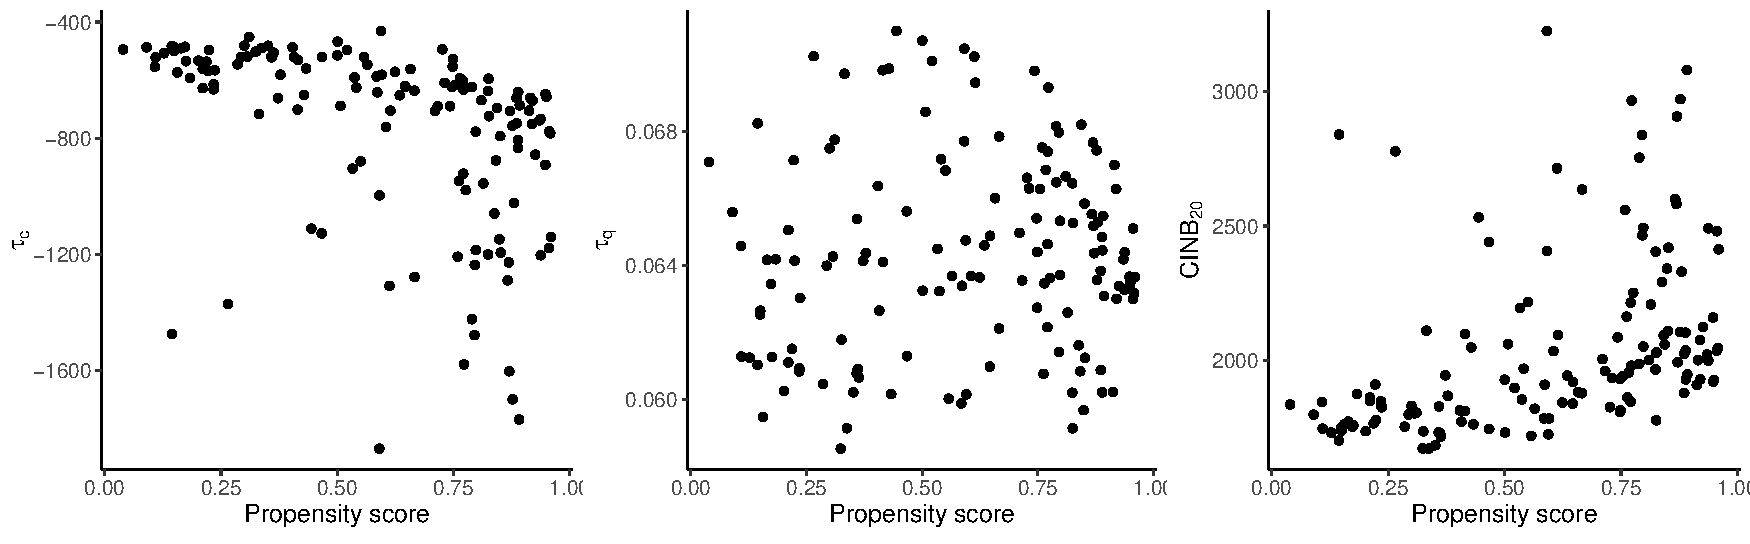
\includegraphics[width=\textwidth]{figures/supplement/CATEplot_ps_v2.pdf}
    \caption{Plots of the estimated propensity scores supplied as a predictor to ps-suBART against the estimated CATE for costs (left), quality (middle), and conditional incremental net benefit at $\lambda=20\mathrm{k}$ (right).}
    \label{fig:CATEplot_ps}
\end{figure}\vspace{-1em}%
\begin{figure}[H]
    \centering
    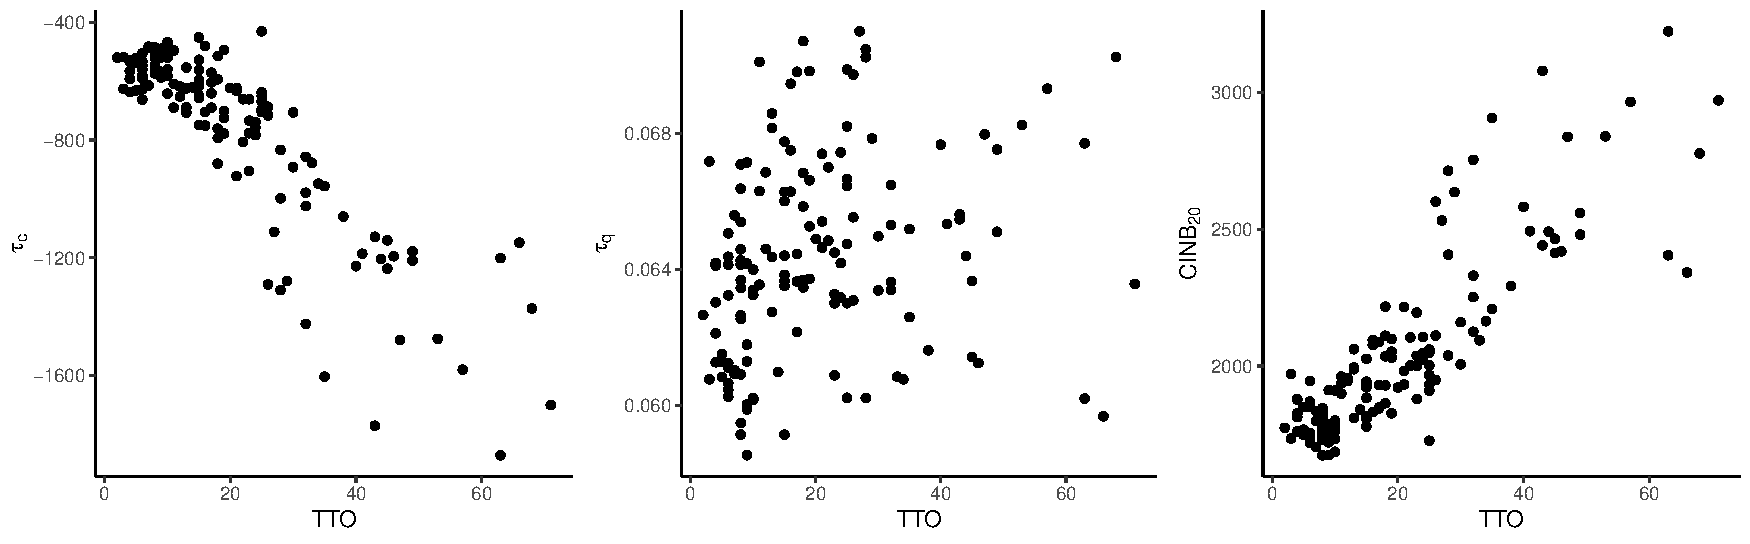
\includegraphics[width=\textwidth]{figures/supplement/CATEplot_TTO_v2.pdf}
    \caption{Plots of the TTO predictor against the estimated CATE for costs (left), quality (middle), and conditional incremental net benefit at $\lambda=20\mathrm{k}$ (right).}
    \label{fig:CATEplot_TTO}
\end{figure}\vspace{-1em}%
\begin{figure}[H]
    \centering
    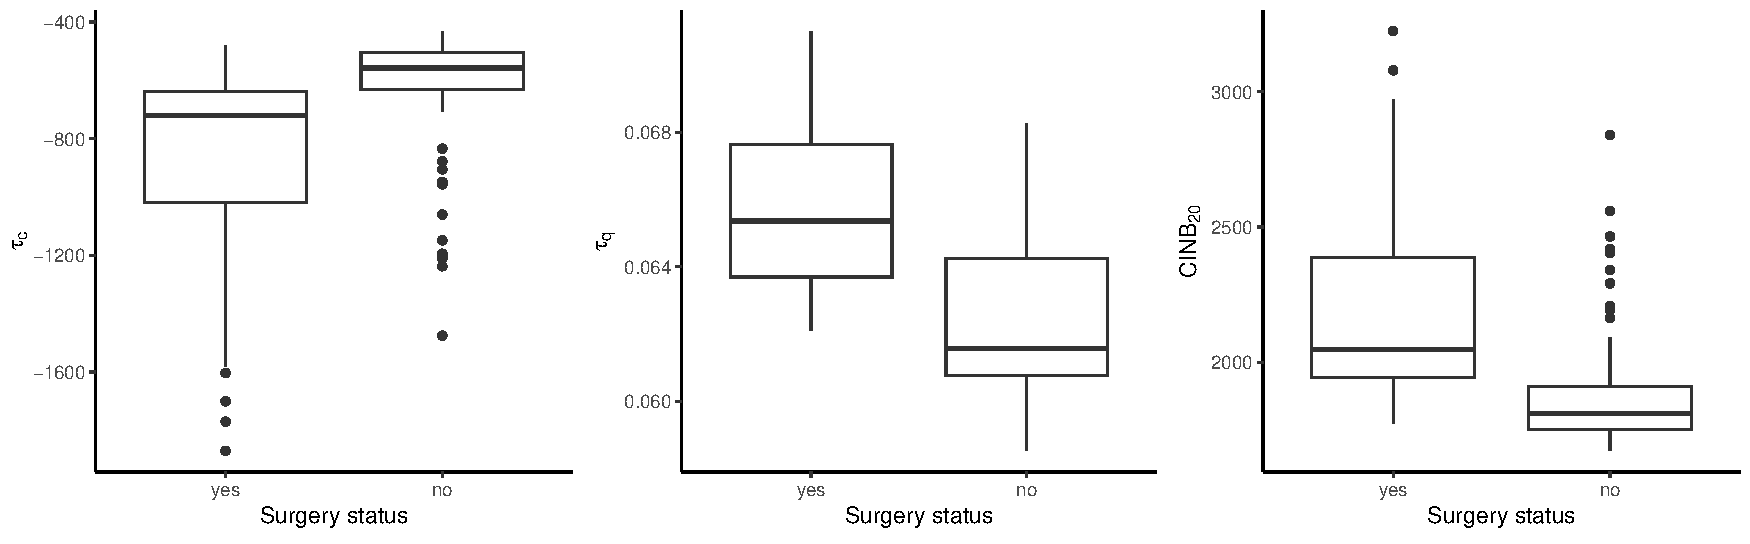
\includegraphics[width=\textwidth]{figures/supplement/CATEplot_surgery_v2.pdf}
    \caption{Box plots of the surgery predictor against the estimated CATE for costs (left), quality (middle), and conditional incremental net benefit at $\lambda=20\mathrm{k}$ (right).}
    \label{fig:CATEplot_surgery}
\end{figure}

Finally, it is also worth noting that the observed heterogeneity in the above plots of $\tau_c(\mathbf{x}_i)$ against various predictors is indicative of non-linearity in $\mathbb{E}\left\lbrack c_i\given t_i, \mathbf{x}_i\right\rbrack$. The same applies to $\tau_q(\mathbf{x}_i)$ and $\operatorname{CINB}_{20\mathrm{k}}(\mathbf{x}_i)$. Thus, there is evidence to support the flexibility of ps-suBART in capturing non-linear relationships.

\subsection{Visualising variable importance}
\label{app:var_imp}

Figure \ref{fig:varimp_plot} shows the percentage of times, averaged across all trees in the outcome-specific ensemble, that a given predictor was used to form a splitting rule for a given outcome in the TTCM application. Similar plots were shown to demonstrate the quantification of variable importance in the original univariate BART setting by \citet{chipman2010bart}. Here, the variable importance scores in Figure \ref{fig:varimp_plot} illustrate the practical implications of a defining feature of suBART, namely that the relative importance of the predictors differs in relation to each outcome. Crucially, this behaviour is achieved without having to pre-specify the functional form of the relationships between the cost and quality outcomes and the available predictors, as a result of BART's intrinsic variable-selection properties. Some interesting findings are worth briefly commenting on. Firstly, we have variables which are important to both outcomes, such as the treatment indicator. Secondly, we have variables which are relatively unimportant for both outcomes, with the hospital admission indicator being the second-least and least used variable, respectively. Thirdly, we have variables which differ in the extent of their importance for each outcome: trauma type is the most used variable for the $c_i$ outcome, while being number six in the ranking for $q_i$. Finally, we note that tailoring the suBART framework to causal inference objectives by supplying propensity scores as a predictor has indeed led to the propensity scores being frequently used to form splitting rules for both outcomes.

\begin{figure}[H]
    \centering
    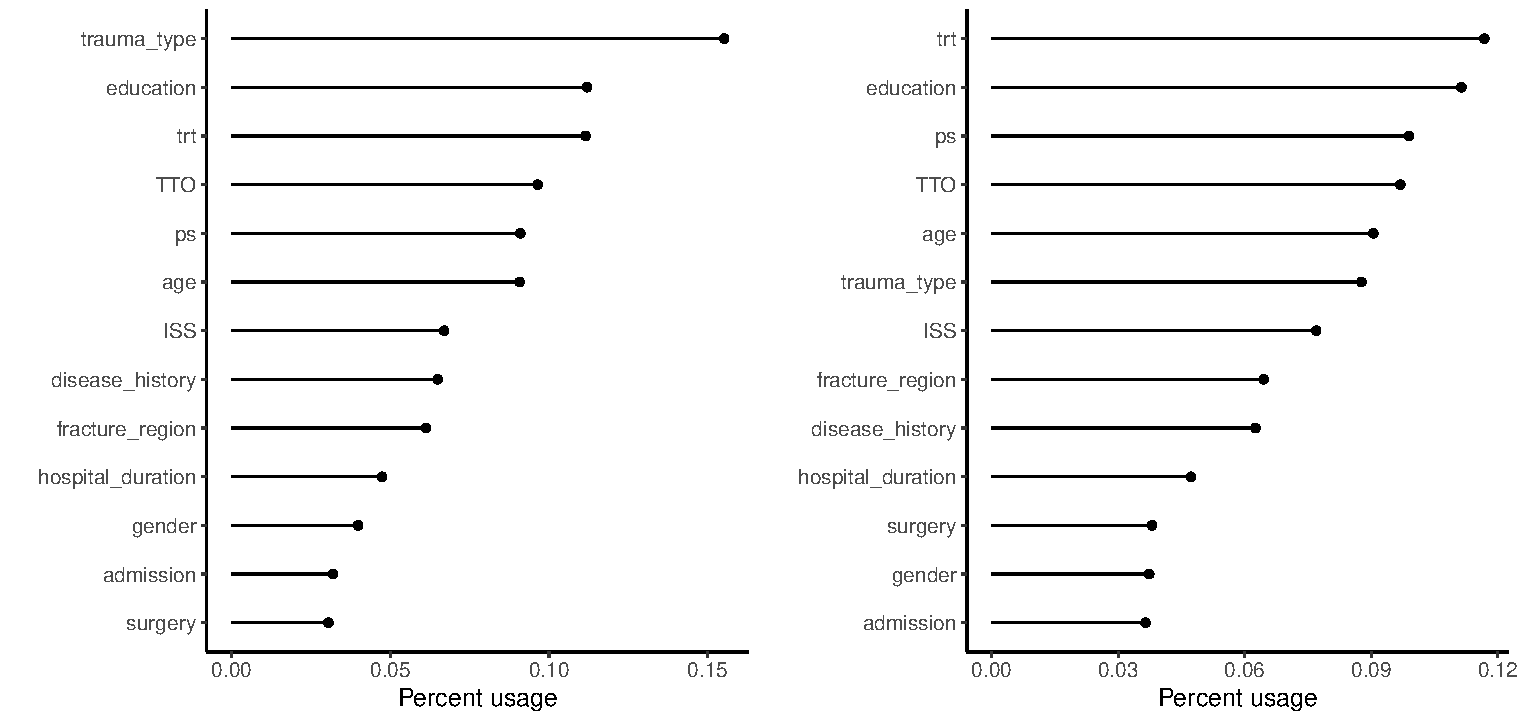
\includegraphics[width=\textwidth]{figures/supplement/varimp_plot.pdf}
    \caption{Average usage of each variable in the TTCM dataset in the 100 trees of the ps-suBART model. The left side shows usage for the outcome $c_i$, while the right shows $q_i$.}
    \label{fig:varimp_plot}
\end{figure}

\section{\textsf{R} scripts}

The \textsf{R} package \texttt{subart} was created to implement the proposed suBART and probit suBART models. Interested readers can find the package available for download from the GitHub repository located at \url{https://github.com/MateusMaiaDS/subart}. A number of \textsf{R} scripts are also provided, both on GitHub and with the online Supplementary Material of this paper, 
in order to reproduce the results throughout the main paper and all Appendices. Finally, the motivating TTCM dataset described in Section \ref{sec:application} is also made publicly available. The following is an overview of the various included files and their purposes:

\begin{itemize}[wide]
    \item \texttt{ttcm.rda}: an abridged and anonymised version of the data from \citet{wiertsema2019cost}, which we used for the analyses throughout Section \ref{sec:case_study}.
    \item \texttt{ttcm\_simulation.r}: the code used for the simulation experiments in Section \ref{sec:TTCM_sim} and Appendix \ref{app:indBART}.
    \item \texttt{ttcm\_application.r}: the code used for the CEA application in Section \ref{sec:TTCM_real_V2} and the additional analyses in Appendix \ref{app:extraTTCM}.
    \item \texttt{stan\_classification\_compile.r}: code to fit the probit version of BayesSUR via \texttt{Stan} \citep{stanusersguide}, through the \textsf{R} interface provided by the \texttt{rstan} package \citep{rstanref}, for the simulation experiments in Section \ref{sec:sim_binary}, along with the additional related results in Appendix \ref{app:friedman}.
    \item \texttt{cv\_functions.r}, \texttt{cv\_results.r}, and \texttt{plot\_simulation\_results.r}: all other code required to fit the remaining models to replicate the Friedman simulation experiments throughout Section \ref{sec:simstudies}, including both the experiments with continuous responses in Section \ref{sec:sim_continuous} and those with binary responses in Section \ref{sec:sim_binary}, along with the additional related results in Appendix \ref{app:convergence} and Appendix \ref{app:friedman}.
\end{itemize}

\end{appendix}

%\clearpage
\interlinepenalty=1000
%\setlength{\bibsep}{3.875pt}
\bibliographystyle{imsart-nameyear}
\bibliography{references}

\end{document}